%HEADER
\documentclass[12pt,letterpaper]{article}

%packages
\usepackage{fixltx2e}
\usepackage{textcomp}
\usepackage{fullpage}
\usepackage{amsfonts}
\usepackage{verbatim}
\usepackage[english]{babel}
\usepackage{pifont}
\usepackage{color}
\usepackage{setspace}
\usepackage{lscape}
\usepackage{indentfirst}
\usepackage[normalem]{ulem}
\usepackage{booktabs}
%\usepackage{nag}
\usepackage{natbib}
%\usepackage{bibtex}
\usepackage{float}
\usepackage{latexsym}
%\usepackage{hyperref} 
\usepackage{url}
%\usepackage{html}
\usepackage{hyperref}
\usepackage{epsfig}
\usepackage{graphicx}
\usepackage{amssymb}
\usepackage{amsmath}
\usepackage{bm}
\usepackage{array}
\usepackage[version=3]{mhchem}
\usepackage{ifthen}
\usepackage{caption}
\usepackage{hyperref}
%\usepackage{xcolor}
\usepackage{amsthm}
\usepackage{amstext} % Add and remove packages as necessary for your manuscript.

%Pagination style and stuff
\linespread{1.66} % All text should be double-spaced with occasional exceptions for tables. 
\raggedright
\setlength{\parindent}{0.5in}

\setcounter{secnumdepth}{0} % Our sections are not numbered and our papers do not have Tables of Contents. We don't present a list of figures or list of tables, either. Any common font is fine. (A common sans-serif font should be used on figures, but figures should be separate from the LaTeX document.)

\pagestyle{empty}

\renewcommand{\section}[1]{%
\bigskip
\begin{center}
\begin{Large}
\normalfont\scshape #1
\medskip
\end{Large}
\end{center}}

\renewcommand{\subsection}[1]{%
\bigskip
\begin{center}
\begin{large}
\normalfont\itshape #1
\end{large}
\end{center}}

\renewcommand{\subsubsection}[1]{%
\vspace{2ex}
\noindent
\textit{#1.}---}

\renewcommand{\tableofcontents}{}

\bibpunct{(}{)}{;}{a}{}{,}  % this is a citation format command for natbib
<<<<<<< HEAD
=======
% We don't use a special title page; the author information is entered like any other text.
% FOOTNOTES: We don't allow them in the manuscript, except in tables. Don't include any footnotes in the text.
%IMPORTANT:
%Note on display in the text file: sentences or sub-parts of sentences (e.g. enumerations) are delimited by a newline for clarity.
%However, true new lines (i.e. in the pdf) are delimited by one or more empty lines.
%We don't use a heading for the introduction. The nature of this section is implied by its position following the abstract and preceding the first major section heading.


>>>>>>> parent of 936e93d... Merge pull request #1 from nhcooper123/master

%---------------------------------------------
%
%       START
%
%---------------------------------------------

\begin{document}

%For a colour version of the draft to a search>replace '-BW'>'' 


%Runing head
\begin{flushright}
Version dated: \today
\end{flushright}
\bigskip
\noindent RH: Missing data and topology in Total Evidence matrices %RH = Running Head

\bigskip
\medskip
\begin{center}

%Title
\noindent{\Large \bf Effect of missing data in matrices containing living and fossil taxa on topological accuracy}
<<<<<<< HEAD
%Alternative punchier title: "Bayesian Total Evidence methods fail to recover correct topologies from matrices containing both living and fossil taxa"
%Alternative punchier title: "Maximum Likelihood outperforms Bayesian methods for inferring topology from Total Evidence matrices containing both living and fossil taxa"

% NC: Not sure about any of these. I actually think I prefer your talk title. So something like: The effects of missing data on the ability of Total Evidence approaches to recover correct tree topologies. No rush to decide. But needs Total Evidence in there somewhere.
=======
%Alternative punch title: "Bayesian method fails to infer topology using matrices containing both living and fossil taxa"
%Alternative punch title: "Maximum Likelihood outperforms Bayesian for inferring topology from matrices containing both living and fossil taxa"
>>>>>>> parent of 936e93d... Merge pull request #1 from nhcooper123/master
\bigskip

%Authors
\noindent {\normalsize \sc Thomas Guillerme$^1$$^,$$^2$, other authors $^3$, and Natalie Cooper$^1$$^,$$^2$}\\
\noindent {\small \it 
$^1$School of Natural Sciences, Trinity College Dublin, Dublin 2, Republic of Ireland;\\
$^2$Trinity Centre for Biodiversity Research, Trinity College Dublin, Dublin 2, Republic of Ireland;\\
$^3$Somewhere else }\\
\end{center}
\medskip
\noindent{\bf Corresponding author:} Thomas Guillerme, School of Natural Sciences, Trinity College Dublin, Dublin 2, Republic of Ireland; E-mail: guillert@tcd.ie.\\
\vspace{1in}

<<<<<<< HEAD
\newpage
\begin{abstract}
% NC: I'm not going to give this much work as it'll change before we submit anyway. Note though that and abstract must NOT just repeat stuff in the intro. Needs rephrasing at the very least.
Living species represent less than 1\% of all species that have ever lived. % NC: I was chatting to Andy Purvis about this the other day and he said lots of palaeo folk hate that stat. So let's not start the abstract with it!
Ignoring fossil taxa may lead to misinterpretation of macroevolutionary patterns and processes such as trends in species richness, biogeographical history or paleoecology.
This fact has led to an increasing consensus among scientists that both living and fossil taxa must be included in macroevolutionary studies.
One approach, the Total Evidence approach, uses molecular data from living taxa and morphological data from both living and fossil taxa to infer phylogenies with both living and fossil taxa at the tips.
Although the Total Evidence approach seems very promising, it requires a lot of data and is therefore likely to suffer from missing data issues which may affect its ability to infer correct phylogenies.
=======

%---------------------------------------------
%
%       ABSTRACT
%
%---------------------------------------------


\subsubsection{Abstract}
Living species represent less than 1\% of all species that have ever lived. Ignoring fossil taxa may lead to misinterpretation of macroevolutionary patterns and processes such as trends in species richness, biogeographical history or paleoecology.
This fact has led to an increasing consensus among scientists that both fossil and living taxa must be included in macroevolutionary studies.
One approach, the total evidence approach, uses molecular data from living taxa and morphological data from both living and fossil taxa to infer phylogenies with both fossil and living taxa at the tips.
Although the total evidence approach seems very promising, it requires a lot of data and is therefore likely to suffer from missing data issues which may affect its ability to infer correct phylogenies.
>>>>>>> parent of 936e93d... Merge pull request #1 from nhcooper123/master

In this study we assess the effect of missing data on tree topologies inferred from Total Evidence matrices.
Using simulations we investigate three major factors that directly affect the completeness of the morphological part of the matrix:
(1) the proportion of living taxa with no morphological data,
(2) the amount of missing data in the fossil record and
(3) the overall number of morphological characters in the matrix.
We find that, in a Bayesian framework, difficulties in recovering a stable topology are mainly driven by the missing data in the molecular part of the matrix (for which fossil taxa have no data).
In a Maximum Likelihood framework, however, topology is not directly affected by missing data \textit{per se}, but by the number of morphological characters shared among the taxa.
Therefore, the two main drivers of incorrect topologies are the overall number of morphological characters and the number of living species with no morphological data.

Our results suggest that, in order to use Total Evidence approaches, one should reduce the missing data in the morphological part of the matrix for living species and use a Maximum Likelihood framework to fix the topology prior to the overall Bayesian phylogenetic inference process.
%More results!

\noindent (Keywords: missing data, Total Evidence, Bayesian, Maximum Likelihood, topology)\\

\vspace{1.5in}

\newpage 


<<<<<<< HEAD
Although most species that have ever lived are now extinct % NC: This avoids giving the dodgy stat of 1%
    \citep{novacek1992ext,raup1993extinction}, the majority of macroevolutionary studies focus solely on living species \citep[e.g.][]{meredithimpacts2011,jetzthe2012}. %or is citing of your own papers in the too "douchebagy" for the second sentence?
% NC: Yeah be careful with self citing. Fine if it's a good fit, but it's totally not here!!! A better citation would be a big biodiversity study, e.g. the bird phylogeny paper.
Ignoring fossil taxa may lead to misinterpretation of macroevolutionary patterns and processes such as the timing of diversification events \citep[e.g.][]{pyrondivergence2011}, relationships among lineages \citep[e.g.][]{manosphylogeny2007} or niche occupancy \citep[e.g.][]{pearmanniche2008}.
This has led to increasing consensus among scientists that fossil taxa must be included in macroevolutionary studies \citep{jacksonwhat2006,quentaldiversity2010,dietlconservation2011,slaterunifying2013,fritzdiversity2013}.
However, to do this we need to be able to place living and fossil taxa into the same phylogenies; a task that remains difficult despite recent methodological developments (e.g. \citealp{pyrondivergence2011,ronquista2012,schragocombining2013}). %Not a nice sentence

Up to now, three main approaches have been used to place both living and fossil taxa % NC: BE consistent. Either living and fossil, or fossil and living. - TG: Let's make it living and fossil then.
    into phylogenies.
These approaches differ mainly in whether they treat fossil taxa as tips or as nodes in the phylogeny, and in which part of the available fossil data is used (i.e. the age of the fossil only or both its age and morphology). % NC: Not sure about bit in brackets - TG: it's the idea of fossil occurence (age) only when node and fossil occurence + topology when tip.
Classical cladistic methods use matrices containing morphological data from both living and fossil taxa and treat each taxon as a tip in the phylogeny.
Relationships among the taxa are then inferred using optimality criteria such as maximum parsimony \citep{simpson1945}.
This approach is commonly used by paleontologists but it ignores the additional molecular data available from living species and does not allow use of probabilistic methods for dealing with phylogenetic uncertainty (but see \citealp{spencerefficacy2013}).
Neontologists, on the other hand, more commonly use probabilistic approaches (e.g. Maximum Likelihood or Bayesian methods) based on matrices containing only molecular data from living species.
Because fossil taxa do not usually have available DNA, fossils are used as nodes rather than tips in these phylogenies and their occurrence age % NC: Need to check the exact phrase needed here. Is it range of occurrence? Occurrence dates? etc. - TG: in paleo jargon we have FAD (first apparition datum) and FOD (first occurrence datum). FAD is always hypothetical (we can't really exactly know when the taxa appeared) and FOD is always subjective (it depends when the fossil was found, maybe next year someone will find another one in older layers). So for the dating, because it's relaxed clock, people use FOD (and also probably because they don't care since it doesn't make a huge difference I guess).
 are used to time calibrate phylogenies \citep{zuckerkandl1965}.
There have been great improvements in the theory and application of these two approaches \citep[e.g.][]{bapsta2013,stadlerdating2013,heaththe2013} as well as much debate about the "best" approach to use \citep[e.g.][]{spencerefficacy2013}.
However neither approach uses all the available data.

A final approach, known as the Total Evidence method, uses matrices containing molecular data from living taxa and morphological data from both living and fossil taxa. %There might be a philosophico-semantic distinction to do here. Is TEM a method or an approach? I'll say that it is an approach because it's more like an idea (put every thing together) than a way to do (how to put everything together). It makes more sense to me compared to a real method e.g. a probabilistic method such as ML where the method states precisely how to do stuff.
% NC: Tricky. Don't think it's too important though. 
% NC: I do think Total Evidence needs capital letters though, like ML and Bayesian - TG: fixed
This approach treats every taxon as a tip in the phylogeny, uses the occurrence age of the fossils to time calibrate the phylogeny, and allows the use of probabilistic methods for estimating phylogenetic uncertainty \citep{eernissetaxonomic1993}.
Total Evidence methods have been successfully applied to empirical data \citep{pyrondivergence2011,ronquista2012,schragocombining2013}, and are becoming an increasingly popular way of adding fossil taxa to phylogenies.
However, although the Total Evidence approach seems very promising, there is one big drawback in using this approach: it requires a lot of data.
%In particular it requires morphological data from both living and fossil taxa, both of which are known to be scarce. % NC: Really? I know fossil data is known to be scarce, but living data? I think people would be surprised. And they are surprised. We were surprised! Needs a citation either way.
%TG: how about this:
The morphological data for living taxa is rarely collected when molecular data is available (e.g. \citealp{O'Leary08022013} vs. \citealp{meredithimpacts2011}), and for fossil taxa, the scarcity of the fossil record only allow to collect the data available (for example, in vertebrates, the solidest parts of the skeleton \citeal{sansomfossilization2013}).
Therefore Total Evidence matrices are likely to contain a lot of missing data that may affect the method's ability to infer correct topologies, branch lengths and support values \citep{salamin2003}. % Trevor: Missing data also influences support values that trend to decrease

% NC: You need to take a bit of time to learn about singular and plural grammar in English. It's something you always do wrong. e.g. The Total Evidence method *uses* this and *its* parameters are as follows. Versus: Total Evidence methods *use* this and *their* parameters are as follows. Sive and I won't be around to correct your English forever. - TG: my French demons are back!


%Paused here - 15/063

=======
%---------------------------------------------
%
%       INTRODUCTION
%
%---------------------------------------------


Living species represent less than 1\% of all species that have ever lived \citep{novacek1992ext,raup1993extinction}.
However, the majority of macroevolutionary studies focus solely on living species \citep{cooperwhat2009,meredithimpacts2011,healyecology2014}. %or is citing of your own papers in the too "douchebagy" for the second sentence?
Ignoring fossil taxa may lead to misinterpretation of macroevolutionary patterns and processes such as timing of diversification events \citep[e.g.][]{pyrondivergence2011}, relationships among lineages \citep[e.g.][]{manosphylogeny2007} or niche occupancy \citep[e.g.][]{pearmanniche2008}.
These factors have led to increasing consensus among scientists that fossil taxa must be included in macroevolutionary studies \citep{jacksonwhat2006,quentaldiversity2010,dietlconservation2011,slaterunifying2013,fritzdiversity2013}.
However, to do this we need to be able to place living and fossil taxa into the same phylogenies which still remains complex despite an increasing number of significant efforts \citep{pyrondivergence2011,ronquista2012,schragocombining2013}. %Not a nice sentence

Up to now, three main approaches have been used for combining fossil and living taxa data in phylogenies.
These approaches differ mainly in whether they treat fossil taxa as tips or as nodes in the phylogeny and on which part of the available data of the fossil is used (i.e. the fossil occurrence age only or both the age and the morphology).
Classical cladistic methods uses matrices containing morphological data from both fossil and living taxa and allows to treat each taxon as a tip in the phylogeny; the relation between the taxa can be inferred using optimal criteria such as the maximum parsimony criterion \citep{simpson1945}.
This approach is commonly used by paleontologists but it ignores the additional molecular data available from living species and doesn't allow to use probabilistic methods to deal with inference uncertainty (but see \citet{spencerefficacy2013}.
Neontologists, on the other hand, more commonly use probabilistic methods (e.g. Maximum Likelihood or Bayesian) based on matrices containing only molecular data from living species.
Because fossil taxa do not usually have available DNA, fossils are used as nodes rather than tips in these analyses and only their occurrence age can be used to time calibrate phylogenies \citep{zuckerkandl1965}.
There have been great improvements in the theory and application of these two approaches \citep[e.g.][]{bapsta2013,stadlerdating2013,heaththe2013} as well as much debate about the "best" approach to use \citep[e.g.][]{spencerefficacy2013}.
However none of them is optimal and uses all the available data.

A final approach, known as total evidence approach use matrices containing molecular data from living taxa and morphological data from both living and fossil taxa. %There might be a philosophico-semantic distinction to do here. Is TEM a method or an approach? I'll say that it is an approach because it's more like an idea (put every thing together) than a way to do (how to put everything together). It makes more sense to me compared to a real method e.g. a probabilistic method such as ML where the method states precisely how to do stuff.
It allows to use probabilistic methods, to treat every taxon as a tip in the phylogeny and to use the occurrence age of the fossil to time calibrate the phylogeny \citep{eernissetaxonomic1993}.
Here we focus on this total evidence approach because they have been recently successfully developed and applied to empirical data \citep{pyrondivergence2011,ronquista2012,schragocombining2013}.  %needs a better justification
Although the total evidence approach seems very promising, there is one big drawback in using this approach: it requires a lot of data.
In particular it requires morphological data form both living and fossil taxa, both of which are known to be scarce.
Therefore total evidence approach is likely to suffer from having lots of missing data which may affect their ability to infer correct topology, branch length and support values \citep{salamin2003}. % Trevor: Missing data also influences support values that trend to decrease
>>>>>>> parent of 936e93d... Merge pull request #1 from nhcooper123/master

The effect of missing data on phylogenetic inferences has been widely studied \citep{wiensmissing2003,wiensmissing2006,wiensmissing2008,lemmonthe2009,rouresite-specific2011,sansomfossilization2013}.
Missing molecular data has been seen by some authors as an issue because it can decrease the phylogenetic signal in some parts of the tree, especially when using large matrices \citep{lemmonthe2009}.
However other authors do not see missing molecular data as a major issue because the phylogenetic signal, rather than by reducing the amount of missing data, is more likely to increase by having:
(i) at least a "modest" number of highly covered genes (i.e. approximatively half of the genes - \citet{rouresite-specific2011});
(ii) a higher number of taxa (especially slowly evolving taxa or taxa close to the outgroup - \citet{rouresite-specific2011}) and
(iii) by choosing more adequate models of sequence evolution rather than by reducing the amount of missing data \citep{wiensmissing2006,wiensmissing2008,rouresite-specific2011}.

Similarly, depending on the study, missing morphological data might be seen as either a major or minor issue for accurately inferring phylogenies depending on the study \citep{wiensmissing2003,sansomfossilization2013}.
Because soft-tissues characters are rarely preserved in the fossil record, missing data is mainly found in soft tissues characters, and is therefore not randomly distributed, which can lead to biased placement of fossil taxa in phylogenies \citep{sansomfossilization2013}.
However, the phylogenetic signal is not related to the level of missing data \textit{per se} but to the number of informative characters per taxa, therefore missing data is less an issue than the number of shared informative characters \citep{wiensmissing2003}.
Although missing data as been shown to be no major problem separately in molecular and morphological matrices \citep{wiensmissing2003,wiensmissing2006,wiensmissing2008,rouresite-specific2011} it may become an issue when combined in a total evidence type matrices.
Because the nature of total evidence matrices, combining both molecular and morphological information for both living and fossil taxa, a big part of the matrix contains only missing data - the molecular data for fossil taxa.
Until now, no attempt has been made to study the impact of this issue on phylogenetic inference and especially on topological recovery.

Here we assess the effect of missing data on tree topology inferred from total evidence matrices.
The molecular part for living taxa of a total evidence matrix acts like a "classical" molecular matrix \citep{ronquista2012}.
The effect of missing data on such matrices is well known \citep{wiensmissing2006,wiensmissing2008,rouresite-specific2011}, therefore, we only focus on the missing data issue in the morphological part of the matrix.
Using simulations we investigate three major factors that directly affect the completeness of the morphological part of the matrix:
(1) the proportion of living taxa with no morphological data,
(2) the amount of missing data in the fossil taxa (i.e. the preservation quality of the fossil record) and
(3) the overall number of morphological characters for both living and fossil taxa in the matrix.
We assess how removing data from a total evidence type matrix by changing the values of these three parameters affects the topology of the inferred tree using Maximum Likelihood and Bayesian method.
%This paragraph is crap

We found that whatever the amount of missing data, total evidence matrices dramatically reduce the performance of Bayesian inference.
However, when using a Maximum Likelihood approach, missing data decreases gradually the ability of recovering the right tree topology.
We propose that this drastic difference between Bayesian and Maximum Likelihood methods is due to a flattening of the likelihood landscape because of the intrinsic amount of missing data in a total evidence matrix (i.e. the missing molecular data for the fossil taxa).
This problem leads to an inability of Bayesian chains to pick up the sub and near optimal topologies leading to high variance in the posterior tree distribution and really low support in the consensus tree.
These results should encourage authors in not using Bayesian inference to explore the topological landscape of their phylogeny.
Instead, we suggest that authors should first find the Maximum Likelihood tree and use it's topology as a fix prior in their Bayesian inference.
We also propose a new method for comparing Bayesian posterior tree distribution's topology available in a wonderful R package. %Or am I just dreaming a bit too much here?

%---------------------------------------------
%
%       METHODS
%
%---------------------------------------------


\section{Methods} %no material needed?
<<<<<<< HEAD
To explore the effect of missing data in total evidence matrices on tree topology we used the following protocol (note that we explain each step in detail below this general outline -Fig. ~\ref{Fig_Outline}):
=======
% NC: Depends on the journal. See what Syst Biol asks for as section titles.
<<<<<<< HEAD
To explore how missing data in the morphological sections of Total Evidence matrices influences tree topology, we used the following protocol (note that we explain each step in detail below this general outline; Fig.~\ref{Fig_Outline}). %NC: does Syst Biol use Fig. or Figure?
>>>>>>> FETCH_HEAD
=======
To explore how missing data in Total Evidence matrices influences tree topology we used the following protocol (note that we explain each step in detail below this general outline; Fig.~\ref{Fig_Outline}). %NC: does Syst Biol use Fig. or Figure?
>>>>>>> parent of 54cd719... Editted draft methods
\begin{enumerate}
\item{Generating the matrix:} \label{step:generate_matrix} \\
We randomly generated birth death tree (hereafter called the "true" tree, Table ~\ref{Tab_glossary}) to infer a matrix containing both molecular and morphological data for living and fossil taxa (hereafter called the "complete" matrix, Table ~\ref{Tab_glossary}).
\item{Removing data:} \label{step:remove_data} \\
We removed data from the morphological part of the "complete" matrix to simulate the effects of missing data by modifying three parameters (1) the proportion of missing living taxa ($M_{L}$), (2) the proportion of missing data in the fossil taxa ($M_{F}$) and (3) the proportion of missing morphological characters ($M_{C}$) (the resulting matrices are called hereafter the "missing-data" matrix, Table ~\ref{Tab_glossary}).
\item{Building phylogenies:} \label{step:build_phylo} \\
We inferred Bayesian phylogenetic trees from the "complete" matrix and from the "missing-data" matrices resulting in respectively a tree generate from a matrix containing no missing data in the morphological part (hereafter called the "best" tree, Table ~\ref{Tab_glossary}) and trees inferred from matrices with missing data in their morphological part (hereafter called the "missing-data" trees, Table ~\ref{Tab_glossary}).
\item{Comparing topologies:} \label{step:compare_topo} \\
We then compared the "best" tree to the "missing-data" trees to assess the influence of each parameter ($M_{L}$, $M_{F}$, $M_{C}$ and their interactions) on the topologies of the phylogenies we estimated.
\end{enumerate}
To measure the effect of missing data distribution, we repeated steps ~\ref{step:generate_matrix} to ~\ref{step:compare_topo} with the exact same fixed parameters 51 (3$\times$17) times. %that's because I had 3 cluster accounts available... If it's a too odd number, no worries, I'll just remove the last chain.
A list of all the terms used in this paper is available in table ~\ref{Tab_glossary}.


\begin{figure}
\centering
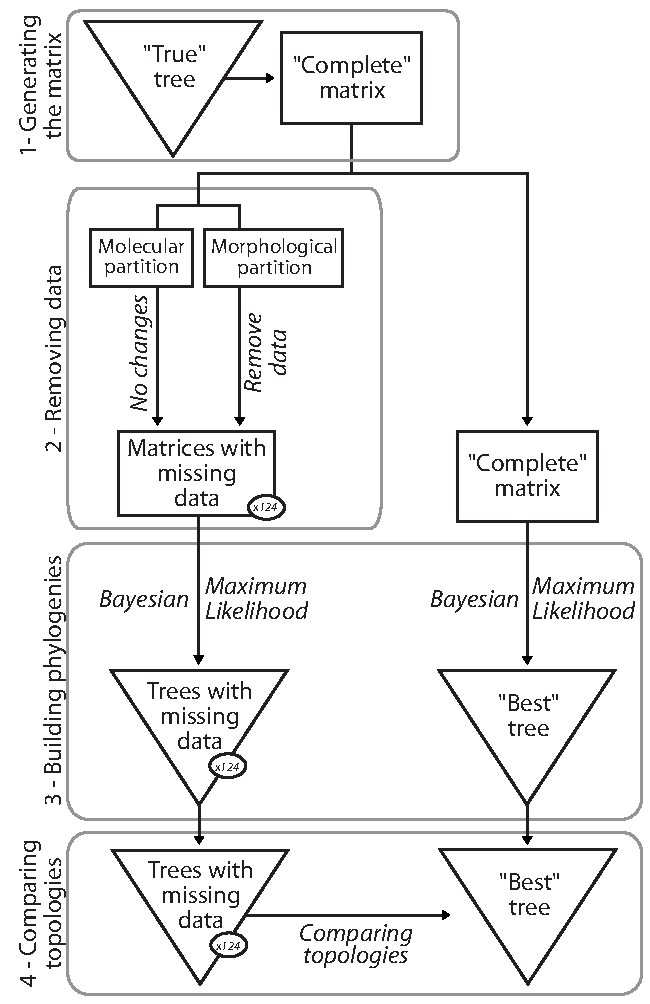
\includegraphics[keepaspectratio=true]{Figures/TEM_Fig_outline-BW.pdf}
\caption{Protocol outline.
(1) We generated a random tree (the "true" tree) to infer a matrix with no missing data (the "complete" matrix).
(2) We removed data from the morphological partition of the "complete" matrix resulting in 125 "missing-data" matrices.
(3) We infer phylogenetic trees from each matrix in both ML and Bayesian framework.
(4) We then compared the "missing-data" trees to the "best" tree.
We repeated step ~\ref{step:generate_matrix} to ~\ref{step:compare_topo} 51 (3$\times $17) times.}
\label{Fig_Outline}
\end{figure}

\begin{table}[ht]
\caption{Glossary}
\centering
\begin{tabular}{p{5cm} p{9cm}}
\hline
\hfill Term & Definition \\[0.5ex]
\hline
\hfill living taxa & taxa with both molecular and morphological data available \\[1.5ex]
\hfill fossil taxa & taxa with only morphological data available \\[1.5ex]
\hfill "complete" matrix & matrix with no missing data except for the molecular part of the fossil taxa \\[1.5ex]
\hfill "missing-data" matrix & matrix with various amount of missing data \\[1.5ex]
\hfill $M_{L}$ & missing living taxa in the morphological part of the matrix \\[1.5ex]
\hfill $M_{F}$ & missing data for the fossil taxa in morphological part of the matrix \\[1.5ex]
\hfill $M_{C}$ & missing morphological characters for both living and fossil taxa \\[1.5ex]
\hfill "true" tree & tree used to simulate the matrix \\[1.5ex]
\hfill "best" tree & tree inferred from the "complete" matrix \\[1.5ex]
\hfill "missing-data" tree & tree inferred the "missing-data" matrices \\[1.5ex]
\hfill RPBTC & Random pairwise Bayesian tree comparison \\[1.5ex]
\hfill "horizontal" sub-matrix & sub-matrix with morphological and molecular characters for living taxa \\[1.5ex]
\hfill "vertical" sub-matrix & sub-matrix with morphological data for both living and fossil taxa \\[1.5ex]
\hfill "corner" sub-matrix & sub-matrix with morphological data for living taxa \\[1.5ex]
\hfill "missing-data" sub-matrix & molecular part of the matrix for the fossil taxa (no data) \\
\end{tabular}
\label{Tab_glossary}
\end{table}

%---------------------------------------------
%       Generating the matrix
%---------------------------------------------

\subsection{Generating the matrix}
First we randomly generated a "true" tree of 50 taxa in R v3.0.2 \citep{R302} using the package diversitree v0.9-6 \citep{fitzjohndiversitree2012}.
We generated the tree using a Birth Death process by sampling the values of the speciation events ($\lambda$) and extinction events ($\mu$) from a uniform distribution but maintaining $\lambda$ $>$ $\mu$ \citep{paradistime-dependent2011}.
We implemented a rejection sampling algorithm to select only random trees with 25 living and 25 fossil taxa. %Justification needed?
We then added a taxa to the resulting Birth-Death tree as the outgroup of the tree.
The mean branch length of the tree was used to separate the outgroup from the rest of the taxa and the branch length leading to the outgroup was set as the sum of the mean branch length and the longest root-to-tip length of the tree.

Next, we created a molecular and a morphological matrix from the "true" tree.
The molecular matrix was inferred from the "true" tree using the package phyclust v0.1-14 \citep{chen2011}.
The matrix was made of 1000 characters sites for 51 taxa and generated using the seqgen algorithm \citep{ranbaut1997seqgen}.
We used the HKY model \citep{HKY85} with a random base frequencies and with the transition/transversion rate of 2 \citep{douadycomparison2003} as parameters for generating the matrix.
The substitution rates were distributed following a gamma distribution with an alpha ($\alpha$) shape of 0.5 \citep{yangamong-site1996}.
We chose a low value of $\alpha$ to reduce the number of sites with high substitution rates, thus avoiding too much homoplasy and a decrease in phylogenetic signal.
These parameters were selected to generate data with no special assumption about how the characters evolved as well as to reduce the computational time required if these parameters were estimated rather than defined (total computational time $>$ 65 CPU years).

We inferred the morphological matrix using the ape package v3.0-11 \citep{paradisape:2004} to generate a matrix of 100 character sites for 51 taxa.
We assigned the number of character states (either 2 or 3) for each morphological character by sampling with a probability of 0.85 for two states characters and 0.15 for three state characters.
These probabilities were selected using the overall distribution of characters states extracted from 100 published empirical morphological matrices (See \hyperref[supplementaries]{supplementaries}).
We then ran an independent discrete character simulation for each character using the "true" tree branch length and topology with the randomly selected number of states (2 or 3) and assuming an equal rate of change (i.e. evolutionary rate) from one character state to an other \citep{Pagel22011994}.
This method allows us to have only two parameters per character: the number of states and the evolutionary rate.
For each character, the evolutionary rate was sampled from a gamma distribution with $\alpha$ = 0.5.
We used a low evolution rate parameter (i.e. $\alpha$) in order to avoid homoplasy in the morphological part of the matrix and create a clear phylogenetic signal \citep{wagner2000,davalosintegrating2014}.

All the molecular information for fossil taxa was replaced by missing data ("?").
Finally, we combined the morphological and molecular matrices obtained from the "true" tree.
Hereafter we call this the "complete" matrix: the matrix with no missing data except for the molecular data of the fossil taxa.

%---------------------------------------------
%       Removing data
%---------------------------------------------

\subsection{Removing data}
Once we obtained the "complete" matrix we modified it to get a set of matrices with missing data. %Ugly sentence
We randomly replaced data with "?" in the morphological part of the matrices according to the following parameters (Fig. ~\ref{Fig_RemoveData}):

\begin{enumerate}
\item{The proportion of living taxa with no morphological data ($M_{L}$): 0\%, 10\%, 25\%, 50\% or 75\%.}
This parameter illustrates the number of living taxa that are present in the molecular part of the matrix but not in the morphological one.
Because of the increasing facility to sequence DNA for living taxa, the number of living taxa with molecular data is highly superior the the number of taxa with molecular and morphological data.
\item{The proportion of missing morphological data across all fossil taxa ($M_{F}$): 0\%, 10\%, 25\%, 50\% or 75\%.}
This parameter illustrates the quality of the fossil record. 
\item{The proportion of missing morphological characters across all taxa (living and fossil - $M_{C}$): 0\%, 10\%, 25\%, 50\% or 75\%. }
This parameter illustrates the number of available morphological characters for both living and fossil taxa.
\end{enumerate}

\begin{figure}
\centering
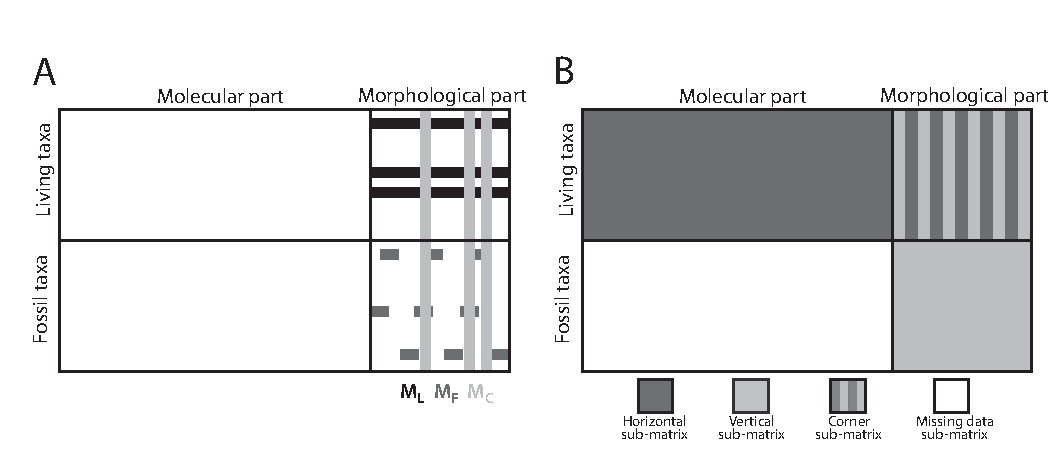
\includegraphics[keepaspectratio=true]{Figures/TEM_Fig_missingData-BW.pdf}
\caption{Names of the different parts of the matrix.
A: Missing data parameters:
Missing living - The proportion of living taxa with no morphological data ($M_{L}$);
Missing fossil - The proportion of missing morphological data across all fossil taxa ($M_{F}$);
Missing character - The proportion of missing morphological characters across all taxa (living and fossil) ($M_{C}$).
B: Different parts of the matrix:
The "horizontal" sub-matrix (orange) contains molecular and morphological data for living taxa;
The "vertical" sub-matrix (blue) contains morphological data for living and fossil taxa;
The "corner" sub-matrix (orange and blue striped) contains morphological data for living taxa;
The "missing-data" sub-matrix (grey) is the molecular part of the fossil taxa and contains no data.}
\label{Fig_RemoveData}
\end{figure}

In practice, each parameter represent a different way of removing data in the morphological part of the matrix: $M_{L}$ removes a proportion of rows from the living taxa; $M_{F}$ removes a proportion of cells from the fossil taxa; and $M_{C}$ removes a proportion of columns across both living and fossil taxa (see Fig. ~\ref{Fig_RemoveData}).
Note that $M_{L}$ is different to $M_{F}$ not only because of the region of the matrix affected: for $M_{L}$, all the morphological data of a proportion of the living taxa is removed (i.e. removing rows), as for $M_{F}$, a proportion of data is removed across the whole of the morphological matrix for fossil taxa (i.e. removing cells).

We tested all parameters combinations resulting in 125 ($5^3$) matrices.
Because some parameter combinations introduce a lot of missing (e.g. $M_L$=75\%, $M_F$=75\% and $M_C$=75\%), some matrices contained fossil taxa without any data at all.
When this occurred we repeated the random deletion of characters until every taxa had at least 5\% data across the whole matrix.

%---------------------------------------------
%       Building phylogenies
%---------------------------------------------

\subsection{Building phylogenies}
From the resulting matrices we generated two types of trees, the "best" tree that is inferred from the "complete" matrix and the "missing-data" trees inferred from the 125 matrices with various amounts of missing data.
The "true" tree was used to generate the "complete" matrix and reflects the "true" evolutionary history in our simulations.
The "best" tree, on the other hand, is the best tree we can build using the state-of-the-art phylogenetic methods.
In real world situations, the "true" tree is never available to us because we cannot know the true evolutionary history of a clade (except in very rare circumstances, e.g. \citet{rozen2005}).
Therefore, here we focus on comparing the trees inferred from the matrices with missing data to the "best" tree, rather than the "true" tree, as the "best" tree is generally what biologists have to work with.

\subsubsection{Maximum Likelihood}
The "best" tree and the "missing-data" trees were inferred using RAxML v8.0.20 \citep{Stamatakis21012014}.
For the molecular data, we used the GTR + $\Gamma_4$ model (\citet{tavare1986}; default GTRGAMMA in RAxML v8.0.20; \citet{Stamatakis21012014}) as a generalisation of the HKY + $\Gamma_4$ model \citep{HKY85} for the molecular data.
The GTR model can be seen as a generalisation of the HKY model (the 2 parameters from the HKY model are implicitly included in the 6 from GTR model - \citet{stamatakisa2008}).
For the morphological data, we used the implemented Markov \textit{k} state model \citep{lewisa2001} which is a generalisation of the JC69 model \citep{jc69} with \textit{k} $\geq$ 2 assuming an equal state frequency and a unique overall substitution rate ($\mu$) following a gamma distribution of the rate variation with four distinct categories (M\textit{k} + $\Gamma_4$; -K MK option in RAxML v8.0.20; \citet{Stamatakis21012014}).
We used the fast bootstrap algorithm and performed 1000 bootstraps per tree inference to assess the topological support. %The explanations of the algorithm part for the BS was proposed by Trevor
The bootstrap algorithm used in RAxML is the Lazy Sub-tree Rearrangement (LSR) which consists in pruning one sub-tree from the tree and subsequently reinserting it to al neighbouring branches \citep{stamatakisa2008}.
Sub-tree Pruning and Reinserting methods (SPR) have been demonstrated as being better than others (e.g. Nearest Neighbouring Interchange - NNI) in recovering good bootstrap values \citep{salamin2003}.

\subsubsection{Bayesian}
The "best" tree and the "missing-data" trees were inferred using MrBayes v3.2.2 \citep{Ronquist2012mrbayes}.
We partitioned the data to treat the molecular part as a non-codon DNA partition and the morphological part as a multi-state morphological partition.
The molecular evolutionary history was inferred using the HKY model with a transition/transversion ratio of two \citep{douadycomparison2003} and a gamma distribution for the rate variation with four distinct categories (HKY + $\Gamma_4$).
For the morphological data, we used the Markov \textit{k} state model \citep{lewisa2001}, with equal state frequency and a unique overall substitution rate ($\mu$) with four distinct rates categories (M\textit{k} + $\Gamma_4$).
We chose these models to be consistent with the parameters used to generate the "complete" matrix.

Each Bayesian tree was estimated using two runs of four chains each for a maximum of 50$\times$$1^6$ generations.
We used the average standard deviation of split frequencies (ASDS) as a proxy to estimate the convergence of the chains and used a stop rule when the ASDS went below 0.01 \citep{Ronquist2012mrbayes}.
The effective sample size (ESS) was also checked on a random sub-sample of runs in each simulation to ensure that ESS $>>$ 200 \citep{drummond2006ess}.
For each run, we removed 25\% of the iterations as burn-in.
We used the following prior for each tree (see \hyperref[supplementaries]{supplementaries}):
\begin{enumerate}
\item
the "true" tree’s topology as a starting tree (with a starting value for each branch length of 1),
\item
an exponential prior on the shape of the gamma distribution of $\alpha$=0.5 for both partitions
\item
and a transition/transversion ratio prior of 2 sampled from a strong beta distribution ($\beta$(80,40)).
\end{enumerate}

We used these prior to speed up the Bayesian process.
These prior biased the way the Bayesian process calculated the branch length by giving non-random starting points and boundaries for the parameters estimation process, however, in this study, we focused on the effect of missing data on the topology and not on the branch length.
Even using these prior, it took 65 CPU years to build 51 sets of 125 Bayesian trees (8 core nodes 2.30GHz clock speed).

%---------------------------------------------
%       Comparing Topologies
%---------------------------------------------

\subsection{Comparing topologies}
<<<<<<< HEAD
<<<<<<< HEAD
We compared the topology of the "missing-data" trees inferred from the matrices with missing data to the "best" tree to measure the effect of the three parameters $M_{L}$, $M_{F}$ and $M_{C}$.
Note that we only investigate differences in topology and not in branch length because the aim of this study is to look at the effect of missing data on the topology of trees inferred from Total Evidence type matrices.
=======
We compared the topology of the "missing-data" trees inferred from the matrices with missing data to the "best" tree to measure the effect of the three parameters $M_{L}$, $M_{F}$ and $M_{C}$.
Note that we only investigate differences in topology and not in branch length because the aim of this study is to look at the effect of missing data on the topology of trees inferred from total evidence type matrices.
>>>>>>> parent of 54cd719... Editted draft methods
To compare the topology of the resulting trees, we used two metrics to assess number of conserved taxa and clades position using respectively the Triples \citep{dobson1975triplets} and the Robinson-Fould \citep{RF1981} distance.
We normalised the two metrics using the Normalised Tree Similarity index \citep{Bogdanowicz2012} to generalise our results for any \textit{n} number of taxa.
The three metrics are detailed below.

\subsubsection{Triples distance ($T_{x,y}$) \citep{dobson1975triplets}}
This metric measures the number of different sub-trees of three taxa between two given trees.
Each triplet can be written as $I_{ijk}$=(\textit{ijk}).
Where $I_{ijk}$ is equal to 0 if the the two triplets (\textit{ijk}) are the same in the two trees otherwise $I_{ijk}$ is equal to 1.
For any rooted binary tree there are only three possible combinations per triplets: ((\textit{j},\textit{k}),\textit{i});, ((\textit{i},\textit{k}),\textit{j}); and ((\textit{i},\textit{j}),\textit{k}); \citep{johnson1998}.
If the trees used are not fully binary, a fourth triplet combination is possible: (\textit{i},\textit{j},\textit{k});.
One can calculate $S_n$, the triplet distance between two trees as:
<<<<<<< HEAD
=======
We compared the topology of the "missing-data" trees to the "best" tree to measure the effect of the three parameters $M_{L}$, $M_{F}$ and $M_{C}$ on tree topology. We used the Triples \citep{dobson1975triplets} metric to assess the number of conserved taxa across trees, and the Robinson-Fould \citep{RF1981} distance to identify conserved clade positions. We then used Normalized Tree Similarity index \citep{Bogdanowicz2012} to generalize our results for any \textit{n} number of taxa. These metrics are described in detail below.
% NC: I moved this around a bit to make it clearer what metric fits where. Remember we need American spellings.
% Also I thought it was triplets distance? Good idea to check...

\subsubsection{Triples distance}
% NC: I've tried to remove the word displaced here, as displaced suggests that you have one correct placement and then are comparing it to other trees. But the general meaning is that the placements differ between trees.
Triples distance ($T_{x,y}$; \citealp{dobson1975triplets}) measures the number of sub-trees made up of three taxa (triplets) that differ between two given trees. Each triplet can be written as $I_{ijk}$=(\textit{ijk}). Where $I_{ijk}$ is equal to zero if the the two triplets (\textit{ijk}) are the same in the two trees otherwise $I_{ijk}$ is equal to one. For any rooted binary tree there are only three possible combinations for each triplet: ((\textit{j},\textit{k}),\textit{i});, ((\textit{i},\textit{k}),\textit{j}); and ((\textit{i},\textit{j}),\textit{k}); \citep{johnson1998}. If the trees used are not fully binary, a fourth triplet combination is possible: (\textit{i},\textit{j},\textit{k}). We can calculate the triplet distance between two trees, $S_n$, as:
>>>>>>> FETCH_HEAD
=======
>>>>>>> parent of 54cd719... Editted draft methods
\begin{equation}
S_n = \sum_{ijk} I_{ijk}
\end{equation}
Where:
\begin{equation}
\sum_{ijk} = \binom{n}{4} = \frac{n!}{4!(n-4)!}
\end{equation}
And where \textit{n} is the number of taxa in both trees (modified from \citet{critchlowthe1996}).
If $S_n$=0, the trees are the same (i.e. no taxa as been displaced).
When $S_n$ = $\binom{n}{4}$, the trees are the most different possible (i.e. every taxa as been displaced).
This metric therefore illustrates the amount of displayed taxa.
It is less sensitive to the placement of individual taxa and to taxa of highly uncertain placement (e.g. fossil taxa) than the Robinson-Foulds metric \citep{critchlowthe1996,johnson1998,wiensmissing2003}.
Therefore we used this metric as a proxy to estimate the robustness of the tree to flying taxa (see \hyperref[supplementaries]{supplementaries}).

\subsubsection{Robinson-Fould distance (\textit{RF}) \citep{RF1981}}
This metric measures the number of shared clades among two trees and therefore illustrates the number of exactly conserved groups among the trees.
The Robinson-Fould distance (also called path difference) between two trees reflects the distance between the distributions of the tips among clades in the two trees \citep{RF1981} and can be expressed as following:
\begin{equation}
RF_{x,y} = N_{x} + N_{y} - 2C_{x,y}
\end{equation}
Where $C_{x,y}$ is the number of clades in common in the two trees.
The minimal value of \textit{C} is 1 if the two trees have the same \textit{n} taxa; the maximal value in \textit{C=n-2}.
This metric is more sensitive to taxa displacement than the Triples metric (i.e. if one taxa gets out of a clade, then the clades are no longer considered as similar - \citet{critchlowthe1996,johnson1998,wiensmissing2003}).
Therefore a low value will show a good clade conservation between two trees and a high value will show a bad recovery of common clades (see \hyperref[supplementaries]{supplementaries}).

\subsubsection{Normalised Tree Similarity \textit{NTS} \citep{Bogdanowicz2012}}
For any tree with \textit{n} taxa compared using a tree distance metric \textit{m}, $NTS_m$ represents the similarity score between the two trees given the expected distance between two random Yule trees with \textit{n} taxa.
Let $\bar{d}_{m,n}$\textit{(rand)} be the average distance between two random Yule trees with \textit{n} taxa and $d_{m,n}$\textit{(x,y)} the distance between the two trees \textit{x} and \textit{y} containing each \textit{n} taxa, then:
\begin{equation}
NTS_{m,n}(x,y)=\frac{\bar{d}_{m,n}(rand) - d_{m,n}(x,y)} {\bar{d}_{m,n}(rand)}
\end{equation}
\textit{NTS} ranges from 1 to -$\infty$.
For any \textit{m},\textit{n} when \textit{NTS}=1, the trees are the same;
when \textit{NTS}=0 the trees are not more different than expected by chance;
when \textit{NTS}$<$0, the trees are more different than expected by chance (see \hyperref[supplementaries]{supplementaries}).

$\newline$

We compared the "missing-data" tree to the "Best" tree for each chain.
For the Maximum Likelihood trees we performed pairwise comparisons between the "Best" tree and the "missing-data" tree (see Table ~\ref{Tab_glossary}) for both the Robinson-Fould and the Triples metric.
We calculated the difference between the trees using the metrics described above by using the TreeCmp java script \citep{Bogdanowicz2012}.
For each metric, we normalized the value using the Normalised Tree Similarity scaled with the mean value of 1000 pairwise random tree comparisons for the same metric and the same number of taxa \textit{n}=51 (see \hyperref[supplementaries]{supplementaries}).
We ran the comparison for every "missing-data" tree in each chain resulting in 51 comparisons for every "missing-data" trees. 
We calculated the mode and the 50\% and 95\% confidence intervals from the resulting distribution using the hdrcde R package (v3.1 – \citet{hdrcde}).

Bayesian tree inference allows to account for the statistical uncertainty of a phylogenetic tree by not using an optimal criterion (c.f. Maximum Likelihood) and gives a tree posterior distribution (c.f. the likeliest tree in ML).
This method has the clear advantage of better dealing with error and uncertainty but it's output (a distribution rather than a single tree) is less practical to use for any further study (but see \citet{healyecology2014}). %Awwwwww yiis!
To avoid this problem, people traditionally use the a consensus tree build on a majority rule in order to summarise a Bayesian tree posterior distribution.
This results into a single tree containing both topological and branch length information as well as support information (i.e. posterior probabilities, e.g. \citet{Ronquist2012mrbayes}).
However, using a Bayesian consensus tree has limitation especially if the resulting consensus tree is not well supported or resolved.
Because the metrics used in this study are used to measure variation in topology between two trees (i.e. taxa placement or clade position), comparing two Bayesian consensus trees is not optimal in picking topological difference signal.
For example, if one of the trees is not resolved at all (i.e. a star tree), comparing it to any other tree (even an other star tree) will not give useful results.
Therefore we used the entire Bayesian trees posterior distribution in order to perform the tree comparisons (i.e. the "Best" Bayesian tree posterior distribution vs. the "missing-data" Bayesian tree posterior distribution).

\subsubsection{Random Pairwise Bayesian Tree Comparison (RPBTC)}
We compared the Bayesian posterior distribution using a Random Pairwise Bayesian Tree Comparison (RPBTC) method.
This method consists in comparing a series of randomly selected pairs of trees from two posterior distributions (on from each distribution) and use the mode to summarize the resulting distribution as a proxy of the difference between the two trees in a Bayesian framework.
\begin{equation}
RPBTC_{X,Y}=Mo[(]d_{m,n}(X_{i1},Y_{j1}),d_{m,n}(X_{i2},Y_{j2}),d_{m,n}(X_{i3},Y_{j3}), ... ,d_{m,n}(X_{ik},Y_{jk})]
\end{equation}

Where \textit{X} and \textit{Y} are two Bayesian tree posterior distributions;
 $d_{m,n}$ is the pairwise difference for any metric \textit{m} and \textit{n} taxa between $X_{i}$ and $Y_{j}$ which are two single trees randomly sampled respectively from \textit{X} and \textit{Y};
 $Mo$ is the mode and
 $Mo[(d_{m,n}(X_{i1},Y_{j1}),d_{m,n}(X_{i2},Y_{j2}),d_{m,n}(X_{i3},Y_{j3}), ... ,d_{m,n}(X_{ik},Y_{jk})]$ is the mode of the pairwise difference repeated \textit{k} times.

We used the mode to summarize the distributions because it is the value that is the most represented in the distribution and reflects what a consensus tree represents (the topology the most represented in the posterior distribution).
Also, the mode is a value present in the distribution (which, depending on the metric, can be a series of discrete values) in contrast to the other distribution summary metrics, such as the mean or the median, which can take values that are not actually present in the distribution.
For example, if comparing two posterior tree distribution, we obtain difference values of 10, 10, 10, 5, 5 and 1, using the mean (6.8) or the median (7.5) gives a values that actually doesn't exist. %Useful?

In this study, we calculated RPBTC for both metrics (Robinson-Fould and Triples distance) for each pairs of Bayesian tree distributions (i.e. the "Best" Bayesian tree posterior distribution vs. the "missing-data" Bayesian tree posterior distribution) with 1000 random pairwise comparisons (\textit{k}).
Because the RPBTC uses random pairwise comparisons, there is a chance of comparing always trees that have the biggest or the smallest difference between two distributions, either deflating or inflating the RPBTC difference value.
However, using 1000 random pairwise comparisons makes the difference stable (i.e. if repeated independently, no difference is detected - see \hyperref[supplementaries]{supplementaries}).

$\newline$

We calculated the NTS for the "Best" Bayesian tree vs. "missing-data" Bayesian tree comparison for both Robinson-Fould and Triples metric using the mode of the RPBTC for each chain resulting in a distribution of 51 modes per comparison.
We then compared the NTS of the Bayesian trees to the NTS of the ML trees for both metrics for each comparison.
This resulted in a distribution of 51 NTS values for the Bayesian trees and 51 NTS values for the ML trees for each tree comparison for which we calculated the mode and the 50\% and 95\% confidence intervals (see \hyperref[supplementaries]{supplementaries} - Fig. ~\ref{Fig_Compare}).

\begin{figure} % Modify the figure
\centering
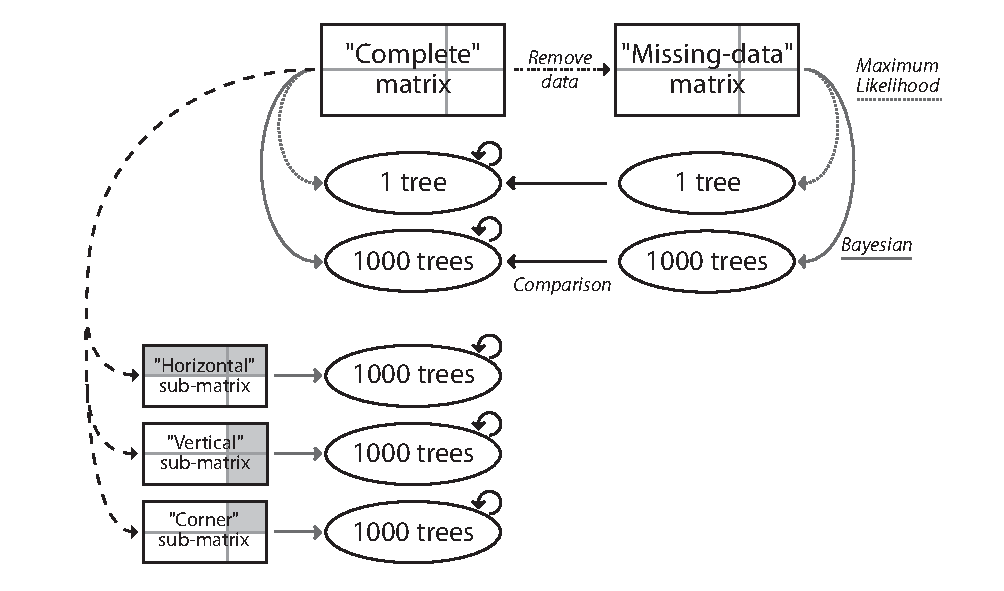
\includegraphics[keepaspectratio=true]{Figures/TEM_Fig_TreeCmp-BW.pdf}
\caption{Tree comparison protocol.
From each of the 125 parameters combination ($M_L$, $M_F$ and $M_C$), we inferred a tree in Baysian or Maximum likelihood framework.
We then compared this tree with or without fossil/living taxa to the "best" tree.
In the Bayesian framework, 1000 trees from the posterior distribution where used for each comparison.}
\label{Fig_Compare}
\end{figure}

\subsubsection{Statistical difference between tree topologies} %note that in the end, I only have non-parametric tests, the parametric explanation part can go to the supplementaries
To assess the difference between the tree topologies, whether they were inferred in a Bayesian or a ML framework, we performed a group comparison test for each set of configurations (e.g. effect of $M_L$ in Bayesian inference, combined effect of $M_F$ and $M_C$ in ML inference, etc...).
We used the pairwise tree comparisons as factors (i.e. the "Best" tree vs. one of each of the 125 "missing-data" trees) and the values of the 51 replicates from the pairwise comparison as a response variable.
The 51 replicates values were either the replicates of the 51 pairwise tree comparisons in ML or the modes of the 51 RPBTC posterior distributions in Bayesian.
When we found a significant difference between the groups, we performed a pairwise comparison test to analyse which pairs of groups differ from the others.
Depending on whether the data was normal with variance homoscedasticity or not (controlled by performing respectively a shapiro.test and a a bartlett.test in R\{stats\}), we used respectively parametric or non-parametric tests for the group comparison and the pairwise comparisons as suggested by \citet{ruxtontime2008} (Table ~\ref{Stats_test}). %link broken

\begin{table}[ht]
\caption{Statistical tests}
\centering
\begin{tabular}{lrll}
  \hline
   & test & statistics & code\{package\} \\ [0.5ex]
  \hline
  Groups comparisons & ANOVA & parametric & anova\{stats\} \\ [0.5ex]
                     & Kruskal-Wallis & non-parametric & kruskal.test\{stats\} \\[0.5ex]
  \hline
  Pairwise comparisons & Tukey HSD & parametric & TukeyHSD\{stats\} \\ [0.5ex]
                       & Nemenyi-Damico-Wolfe-Dunn & non-parametric & kruskalmc\{pgirmess\} \\ [0.5ex]
  \hline
\end{tabular}
\label{Stats_test}
\end{table}

\subsection{Effect of missing molecular characters for fossil taxa} %Awfull name.
To assess the effect of missing molecular characters for fossil taxa in a Bayesian framework, we split the "complete" matrix in sub-matrices containing no missing data at all (see Fig. ~\ref{Fig_RemoveData}):
\begin{enumerate}
\item
A first containing both molecular and morphological data for living taxa only (hereafter called the "horizontal" sub-matrix, Table ~\ref{Tab_glossary});
\item
A second one containing morphological data for both living and fossil taxa (hereafter called the "vertical" sub-matrix, Table ~\ref{Tab_glossary});
\item
A third one containing morphological data for living taxa only (hereafter called the "corner" sub-matrix, Table ~\ref{Tab_glossary});
\end{enumerate}
We reran the Bayesian tree inference on the different sub-matrices with no missing data in the same way as described above.
We then compared the resulting tree posterior distribution to itself (in the same way described above) to assess the ability to recover topology for each simulation when no missing data was involved in the phylogenetic inference process.

%---------------------------------------------
%       Empirical data - TO DO
%---------------------------------------------

\subsection{Empirical data} %Still not done!
We also compared the results obtained from simulated data by using \citet{ronquista2012} empirical data.
The matrix contains 67 living species plus one outgroup and 45 fossil species of Hymenopteras with 5097 molecular characters and 354 morphological characters.
From the 68 living species used in the matrix, only 66 had molecular data, we therefore treated these 66 taxa as "living" taxa and all the other 47 as "fossil" taxa.
We treated the matrix in the exact same way as described in step 2 and 3 resulting in 125 matrices with various amount of missing data and the same number of Maximum Likelihood and Bayesian trees.
We used the same settings as for the simulated data in the Maximum Likelihood framework.
For the Bayesian inferences however, we didn’t used any priors except that we provided a starting tree with the topology of the 68 living species (topology with the highest posterior probability from non-clock analysis - \citet{ronquista2012}).
Contrary to \citet{ronquista2012} analysis, we didn’t performed any clock analysis since we were only interested in the topology of the inferred tree and not the branch length.


%---------------------------------------------
%
%       RESULTS
%
%---------------------------------------------


\section{Results}

\subsection{Building the trees}
When generating the matrices using seqgen \citep{ranbaut1997seqgen} and rTraitDisc \citep{paradisape:2004} algorithms with low evolutionary rate parameter ($\alpha$=0.5) we successfully generated evolutionary histories.
In Maximum Likelihood, support values ranged from 0 to 100 with a median of 38 ($1^st$ quartile = 14, $3^rd$ quartile = 72 - see \hyperref[supplementaries]{supplementaries}). % This is actually bad.
The distribution of the phylogenetic signal across the different chains provided us a good spread of evolutionary scenarios: from well resolved phylogenies to poorly resolved ones.
This allows us to test our simulations in a theoretical as well as practical framework (i.e. phylogenies with low support values are rarely published but are still common in early stages of projects). %REF??? - That's kind of my way to turn these bad results into something usable: even if some of our simulations are not realistic, it shows the effect of missing data in any scenario possible, not only in realistic cases.
Also, one can advocate that this low topological resolution is actively due to the amount of missing data in the Total Evidence matrices since the sub-matrices (no missing data) analysis recovers way higher support value  . %This is something that I will had with the whole submatrices story. Basically, when you have all the fossil/molecular data missing, it's harder to build the tree, both in ML and in Bayesian. When you run the analysis without missing data, then it works way better (i.e. our REAL control test: can we simulate matrices in the first place).
Using Bayesian inference, all the chains converged with a significant effective sample size by using 2 parallel runs of 4 chains each (ASSD $<$ 0.01 and ESS $>>$ 200 for inference).

%\subsection{Comparing topologies}
%Did it worked? See sub-matrices part. TO DO

\subsection{Effect of the missing data parameters}

%10/06 - Missing 8 ML Chains
\begin{figure} 
\centering
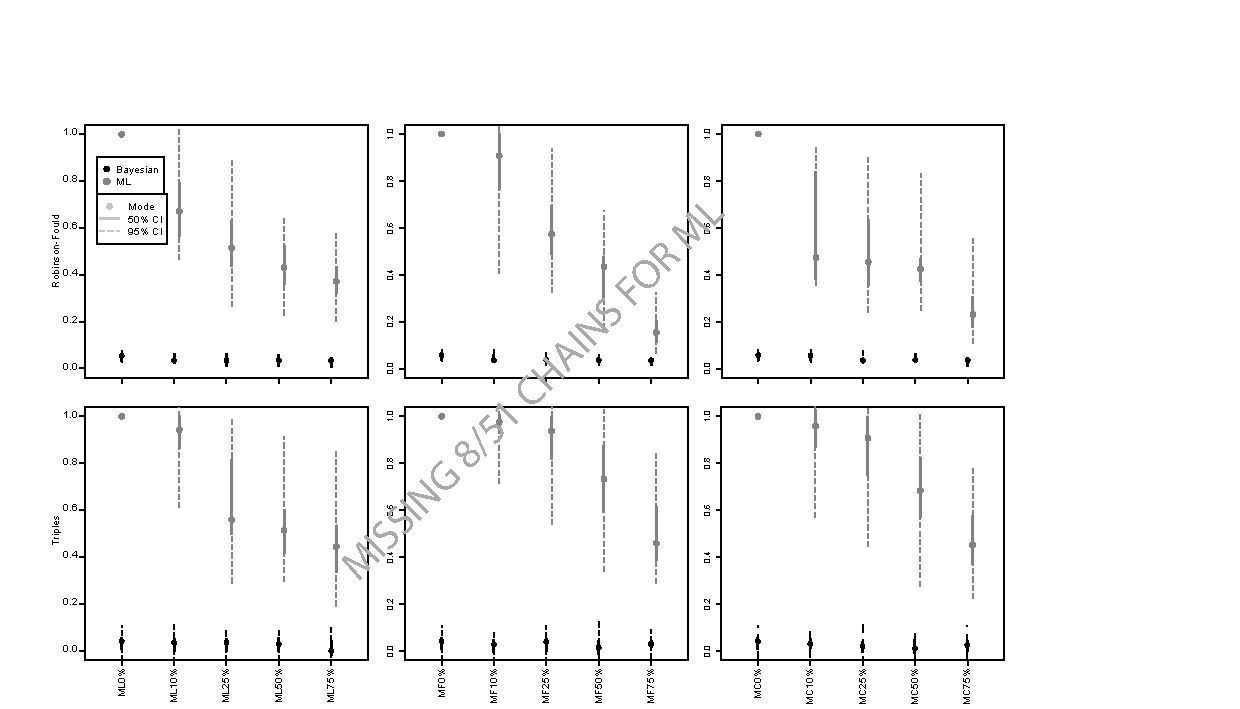
\includegraphics[keepaspectratio=true]{Figures/TEM_Fig-results-BW.pdf}
\caption{Effect of missing data on Tree similarity.
$M_L$ is the amount of missing living taxa with morphological data,
$M_F$ is the amount of missing data in the fossil record,
$M_C$ is the amount of missing morphological characters.
The first row represent the Normalised Tree Similarity index using the Robinson-Fould metric;
the second row represent the Normalised Tree Similarity index using the Triples metric.}
\label{Fig_Results}
\end{figure}


\subsubsection{Effect of $M_L$}
In Maximum Likelihood framework, the topological recovery (reflected by the tree similarity) quickly drops with the increasing amount of missing data when using both metrics (see Table ~\ref{Group_results} - Fig. ~\ref{Fig_Results}).
However, this negative effect of missing data is stabilized beyond 25\% of missing data (no significant difference for trees with respectively 25\%, 50\% and 75\% missing living taxa).
With 10\% of missing living taxa, there is a different topological recovery depending on the used metric.
The Robinson-Fould metric shows a lower Tree similarity index than the Triples metric meaning that individual taxa position are generally more conserved (i.e. low number of flying taxa) but that the full clades are less conserved (see Table ~\ref{NTS_ML_results}).

However, topological recovery was bad in Bayesian, regardless the amount of missing data.
The tree similarity index was only slightly above 0 which means that the mode of the RPBTC was only slightly different than expected by chance (see Table ~\ref{NTS_Ba_results}).
Even if the topological recovery is really low, we detected an effect of missing data on the topology depending on the used metric.
For the Triples metric there is no significant effect of the $M_L$ parameter, in other words, if living taxa are removed, there is no effect on the placement of "flying" taxa.
For the Robinson-Fould metric, there is a significant effect of the $M_L$ leading small decrease in topological recovery when $M_L$ increases (see Table ~\ref{Ba_RF-ML_results}).
However, in both cases, the effect of the parameter $M_L$ is still minimal compared to trees generated in a ML framework since the tree similarity index was only slightly higher than expected by chance (see Table ~\ref{Group_results} - Fig. ~\ref{Fig_Results}).

\subsubsection{Effect of $M_F$}
In Maximum Likelihood framework, the effect of missing data in the fossil record appeared to be constant and led to a constant decrease in topological recovery when the missing data increased (see Table ~\ref{Group_results} - Fig. ~\ref{Fig_Results}).
The difference between the two metrics used is more important than for the $M_L$ parameter: clades are less conserved than individual taxa placement as the amount of missing data increases.
Interestingly, 10\% or 25\% missing data for the $M_F$ parameter does not seems to affect the apparition of unstable taxa (Triples NTS modes of respectively 0.97 and 0.93 - Table ~\ref{NTS_ML_results}).

Similarly than for the effect of $M_L$, Bayesian tree recovery was only slightly better than expected by chance.
In the same way as described above, there seems to be a small difference depending on the metric used.
There is no significant effect of the $M_F$ parameter when using the Triplet metric but the effect is significant when using the Robinson-Fould metric (see Table ~\ref{Ba_RF-MF_results}).
However, as mentioned previously the effect of the parameter $M_F$ is still minimal in a Bayesian framework (see Table ~\ref{Group_results} - Fig. ~\ref{Fig_Results}).

\subsubsection{Effect of $M_C$}
The number of missing morphological characters ($M_C$), however, seems to be more affecting topological recovery than $M_L$ and $M_F$ (see Table ~\ref{Group_results} - Fig. ~\ref{Fig_Results}).
The Robinson-Fould metric shows a rapid drop in tree recovery from 10\% of missing data (Robinson-Fould NTS mode $<$ to 0.5 from 10\% missing data - Table ~\ref{NTS_ML_results}).
This decrease is however slower when using the Triples metric with still a good topological recovery at 10\%  (Triples NTS modes = 0.95 - Table ~\ref{NTS_ML_results}).

The effect of $M_C$ in Bayesian framework is similar as the one described for $M_L$ and $M_F$: tree recovery is only slightly better than expected by chance and only the Robinson-Fould metric shows a significant effect of the $M_C$ parameter on tree recovery (see Table ~\ref{Ba_RF-ML_results} and ~\ref{Group_results} - Fig. ~\ref{Fig_Results}).

%\subsubsection{Combined effect}
%Need to do the heat plots

$\newline$

%To sum up:
The ability of recovering the "best" tree's topology in Maximum Likelihood method is function of the amount of data missing.
The parameters $M_C$ and $M_L$ have more influence than $M_F$ on decrease in topological recovery.
The decrease in clade conservation (low Robinson-Fould NTS score) is faster than the increase in flying taxa (low Triples NTS score).
In Bayesian framework, topology is badly (if not at all) recovered disregarding the amount of data missing.


\begin{table} % What about making this table in a longevity-results style? with every thing combined (30 columns)?
\caption{Tree similarity values per parameter in ML framework}
\centering
\begin{tabular}{rrlccccc}
    \hline
    Parameter & amount of    & metric & mode & 50\%CI &       & 95\%CI &       \\
              & missing data &        &      & lower  & upper & lower  & upper \\
    \hline
    $M_L$     & 0\%          & Robinson-Fould & 1 & NA  & NA & NA  & NA \\
              &              & Triples        & 1 & NA  & NA & NA  & NA \\
              & 10\%         & Robinson-Fould & 0.671 & 0.569  & 0.789 & 0.468  & 1.036 \\ %how many digits?
              &              & Triples        & 0.942 & 0.868  & 0.999 & 0.612  & 1.063 \\
              & 25\%         & Robinson-Fould & 0.516 & 0.440  & 0.630 & 0.266  & 0.892 \\
              &              & Triples        & 0.559 & 0.708  & 0.810 & 0.291  & 0.999 \\
              & 50\%         & Robinson-Fould & 0.432 & 0.364  & 0.521 & 0.231  & 0.642 \\
              &              & Triples        & 0.514 & 0.419  & 0.599 & 0.293  & 0.910 \\
              & 75\%         & Robinson-Fould & 0.372 & 0.323  & 0.434 & 0.203  & 0.577 \\
              &              & Triples        & 0.444 & 0.338  & 0.532 & 0.192  & 0.855 \\
    $M_L$     & 0\%          & Robinson-Fould & 1 & NA  & NA & NA  & NA \\
              &              & Triples        & 1 & NA  & NA & NA  & NA \\
              & 10\%         & Robinson-Fould & 0.907 & 0.766  & 1.000 & 0.407  & 1.047 \\
              &              & Triples        & 0.976 & 0.944  & 1.003 & 0.715  & 1.104 \\
              & 25\%         & Robinson-Fould & 0.572 & 0.488  & 0.692 & 0.325  & 0.936 \\
              &              & Triples        & 0.937 & 0.820  & 0.993 & 0.539  & 1.086 \\
              & 50\%         & Robinson-Fould & 0.433 & 0.302  & 0.476 & 0.170  & 0.668 \\
              &              & Triples        & 0.732 & 0.594  & 0.873 & 0.341  & 1.025 \\
              & 75\%         & Robinson-Fould & 0.153 & 0.115  & 0.200 & 0.068  & 0.323 \\
              &              & Triples        & 0.458 & 0.390  & 0.611 & 0.290  & 0.856 \\   
    $M_L$     & 0\%          & Robinson-Fould & 1 & NA  & NA & NA  & NA \\
              &              & Triples        & 1 & NA  & NA & NA  & NA \\
              & 10\%         & Robinson-Fould & 0.473 & 0.384  & 0.835 & 0.356  & 0.958 \\
              &              & Triples        & 0.959 & 0.869  & 1.026 & 0.572  & 1.067 \\
              & 25\%         & Robinson-Fould & 0.454 & 0.357  & 0.630 & 0.242  & 0.916 \\
              &              & Triples        & 0.907 & 0.751  & 0.997 & 0.446  & 1.070 \\
              & 50\%         & Robinson-Fould & 0.424 & 0.375  & 0.466 & 0.249  & 0.828 \\
              &              & Triples        & 0.683 & 0.571  & 0.822 & 0.277  & 1.008 \\
              & 75\%         & Robinson-Fould & 0.230 & 0.177  & 0.302 & 0.108  & 0.567 \\
              &              & Triples        & 0.451 & 0.373  & 0.572 & 0.224  & 0.791 \\
    \hline
\label{NTS_ML_results}
\end{tabular}
\end{table}

\begin{table} % What about making this table in a longevity-results style? with every thing combined (30 columns)?
\caption{Tree similarity values per parameter in Bayesian framework}
\centering
\begin{tabular}{rrlccccc}
    \hline
    Parameter & amount of    & mode & 50\%CI &       & 95\%CI & \\
              & missing data &      & lower  & upper & lower  & upper \\
    \hline
    $M_L$     & 0\%          & Robinson-Fould & 0.056 & 0.035  & 0.063 & 0.031   & 0.076 \\ %how many digits?
              &              & Triples        & 0.041 & 0.008  & 0.054 & -0.039  & 0.106 \\
              & 10\%         & Robinson-Fould & 0.035 & 0.035  & 0.035 & 0.028   & 0.061 \\
              &              & Triples        & 0.033 & 0.003  & 0.049 & -0.049  & 0.117 \\
              & 25\%         & Robinson-Fould & 0.035 & 0.035  & 0.035 & 0.015   & 0.061 \\
              &              & Triples        & 0.035 & 0.002  & 0.049 & -0.041  & 0.096 \\
              & 50\%         & Robinson-Fould & 0.035 & 0.035  & 0.035 & 0.015   & 0.056 \\
              &              & Triples        & 0.028 & 0.003  & 0.052 & -0.038  & 0.092 \\
              & 75\%         & Robinson-Fould & 0.035 & 0.035  & 0.035 & 0.010   & 0.043 \\
              &              & Triples        & -0.001 & -0.018 & 0.040 & -0.060 & 0.106 \\
    $M_L$     & 0\%          & Robinson-Fould & 0.056 & 0.035  & 0.063 & 0.031   & 0.076 \\
              &              & Triples        & 0.041 & 0.008  & 0.054 & -0.039  & 0.106 \\
              & 10\%         & Robinson-Fould & 0.035 & 0.031  & 0.056 & 0.027   & 0.076 \\
              &              & Triples        & 0.026 & 0.002  & 0.050 & -0.046  & 0.105 \\
              & 25\%         & Robinson-Fould & 0.035 & 0.035  & 0.035 & 0.0153  & 0.068 \\
              &              & Triples        & 0.038 & 0.002  & 0.050 & -0.046  & 0.105 \\
              & 50\%         & Robinson-Fould & 0.035 & 0.035  & 0.035 & 0.015   & 0.058 \\
              &              & Triples        & 0.014 & -0.011 & 0.039 & -0.038  & 0.124 \\
              & 75\%         & Robinson-Fould & 0.035 & 0.035  & 0.035 & 0.015   & 0.041 \\
              &              & Triples        & 0.029 & 0.019  & 0.042 & -0.030  & 0.089 \\   
    $M_L$     & 0\%          & Robinson-Fould & 0.056 & 0.035  & 0.063 & 0.031   & 0.076 \\
              &              & Triples        & 0.041 & 0.008  & 0.054 & -0.039  & 0.106 \\
              & 10\%         & Robinson-Fould & 0.056 & 0.035  & 0.059 & 0.0281  & 0.076 \\
              &              & Triples        & 0.030 & 0.011  & 0.048 & -0.024  & 0.094 \\
              & 25\%         & Robinson-Fould & 0.035 & 0.035  & 0.035 & 0.023   & 0.076 \\
              &              & Triples        & 0.020 & -0.001 & 0.037 & -0.060  & 0.109 \\
              & 50\%         & Robinson-Fould & 0.035 & 0.035  & 0.035 & 0.030   & 0.059 \\
              &              & Triples        & 0.010 & -0.005 & 0.045 & -0.036  & 0.104 \\
              & 75\%         & Robinson-Fould & 0.035 & 0.035  & 0.035 & 0.011   & 0.043 \\
              &              & Triples        & 0.024 & 0.001  & 0.042 & -0.037  & 0.104 \\
    \hline
\label{NTS_BA_results}
\end{tabular}
\end{table}




\begin{table}
\caption{Group difference per configuration set}
\centering
\begin{tabular}{rllcccc}
    \hline
    set & metric & framework & parametric & $stats^1$ & df & p.value \\
    \hline
    $M_L$         & Robinson-Fould & ML       & no & 151.438  & 4   & \textbf{0.00} \\ %10/06 - Missing 8 ML Chains - 1.001278e-31
                  &                & Bayesian & no & 65.62    & 4   & \textbf{0.00} \\ 
                  & Triples        & ML       & no & 142.8329 & 4   & \textbf{0.00} \\ %10/06 - Missing 8 ML Chains  - 6.983434e-30
                  &                & Bayesian & no & 4.56     & 4   & 0.34          \\ 
    $M_F$         & Robinson-Fould & ML       & no & 179.9238 & 4   & \textbf{0.00} \\ %10/06 - Missing 8 ML Chains - 7.743067e-38
                  &                & Bayesian & no & 85.61    & 4   & \textbf{0.00} \\
                  & Triples        & ML       & no & 150.059  & 4   & \textbf{0.00} \\ %10/06 - Missing 8 ML Chains - 1.977386e-31
                  &                & Bayesian & no & 3.01     & 4   & 0.56          \\
    $M_C$         & Robinson-Fould & ML       & no & 151.3818 & 4   & \textbf{0.00} \\ %10/06 - Missing 8 ML Chains - 1.029428e-31
                  &                & Bayesian & no & 64.23    & 4   & \textbf{0.00} \\
                  & Triples        & ML       & no & 138.374  & 4   & \textbf{0.00} \\ %10/06 - Missing 8 ML Chains - 6.290979e-29
                  &                & Bayesian & no & 26.13    & 24  & 0.35          \\
    $M_L+M_F$     & Robinson-Fould & ML       & no & 734.9213 & 24  & \textbf{0.00} \\ %10/06 - Missing 8 ML Chains - 1.104542e-139
                  &                & Bayesian & no & 317.97   & 24  & \textbf{0.00} \\
                  & Triples        & ML       & no & 531.5558 & 24  & \textbf{0.00} \\ %10/06 - Missing 8 ML Chains - 4.581065e-97
                  &                & Bayesian & no & 3.01     & 24  & 0.56          \\
    $M_L+M_C$     & Robinson-Fould & ML       & no & 542.3233 & 24  & \textbf{0.00} \\ %10/06 - Missing 8 ML Chains - 2.619808e-99
                  &                & Bayesian & no & 290.10   & 24  & \textbf{0.00} \\
                  & Triples        & ML       & no & 437.7413 & 24  & \textbf{0.00} \\ %10/06 - Missing 8 ML Chains -  1.28493e-77
                  &                & Bayesian & no & 22.19    & 24  & 0.57          \\
    $M_F+M_C$     & Robinson-Fould & ML       & no & 812.206  & 24  & \textbf{0.00} \\ %10/06 - Missing 8 ML Chains - 5.463138e-156
                  &                & Bayesian & no & 385.96   & 24  & \textbf{0.00} \\
                  & Triples        & ML       & no & 528.9215 & 24  & \textbf{0.00} \\ %10/06 - Missing 8 ML Chains - 1.619383e-96
                  &                & Bayesian & no & 20.23    & 24  & 0.68          \\ 
    $M_L+M_F+M_C$ & Robinson-Fould & ML       & no & 3603.808 & 124 & \textbf{0.00} \\ %10/06 - Missing 8 ML Chains -3.819574e-169
                  &                & Bayesian & no & 1167.40  & 124 & \textbf{0.00} \\
                  & Triples        & ML       & no & 2047.923 & 124 & \textbf{0.00} \\ %10/06 - Missing 8 ML Chains 
                  &                & Bayesian & no & 115.86   & 124 & 0.69          \\
    \hline
\label{Group_results}
\end{tabular}

$^1$ F-value for parametric tests and Kruskal Wallis $chi^2$ for non parametric tests.
\end{table}

\begin{table}
\caption{$M_L$ non-parametric pairwise difference for Robinson-Fould metric in ML framework} %10/06 - Missing 8 ML Chains
\centering
\begin{tabular}{c|ccccc}
    \hline
              & $M_L$00\% & $M_L$10\% & $M_L$25\% & $M_L$50\% & $M_L$75\% \\
    \hline
    $M_L$00\% & - & \textbf{TRUE}  & \textbf{TRUE} & \textbf{TRUE} & \textbf{TRUE}\\
    $M_L$10\% & & - & \textbf{TRUE}  & \textbf{TRUE} & \textbf{TRUE} \\
    $M_L$25\% & & & - & FALSE  & \textbf{TRUE} \\
    $M_L$50\% & & & & - & FALSE  \\
    $M_L$75\% & & & & & - \\
    \hline
\end{tabular}
\centering
\begin{tabular}{rrrl}
 pairwise comparison & obs.dif & critical.dif & difference \\ 
  \hline
  $M_L$00\%-$M_L$10\% & 56.53 & 37.66 & TRUE \\ 
  $M_L$00\%-$M_L$25\% & 96.85 & 37.66 & TRUE \\ 
  $M_L$00\%-$M_L$50\% & 127.03 & 37.66 & TRUE \\ 
  $M_L$00\%-$M_L$75\% & 144.58 & 37.66 & TRUE \\ 
  $M_L$10\%-$M_L$25\% & 40.31 & 37.66 & TRUE \\ 
  $M_L$10\%-$M_L$50\% & 70.50 & 37.66 & TRUE \\ 
  $M_L$10\%-$M_L$75\% & 88.05 & 37.66 & TRUE \\ 
  $M_L$25\%-$M_L$50\% & 30.19 & 37.66 & FALSE \\ 
  $M_L$25\%-$M_L$75\% & 47.73 & 37.66 & TRUE \\ 
  $M_L$50\%-$M_L$75\% & 17.55 & 37.66 & FALSE \\ 
   \hline
\end{tabular}
\label{ML_RF-ML_results}
\end{table}


\begin{table}
\caption{$M_L$ non-parametric pairwise difference for Triples metric in ML framework} %10/06 - Missing 8 ML Chains
\centering
\begin{tabular}{c|ccccc}
    \hline
              & $M_L$00\% & $M_L$10\% & $M_L$25\% & $M_L$50\% & $M_L$75\% \\
    \hline
    $M_L$00\% & - & \textbf{TRUE}  & \textbf{TRUE} & \textbf{TRUE} & \textbf{TRUE}\\
    $M_L$10\% & & - & \textbf{TRUE}  & \textbf{TRUE} & \textbf{TRUE} \\
    $M_L$25\% & & & - & FALSE  & FALSE \\
    $M_L$50\% & & & & - & FALSE  \\
    $M_L$75\% & & & & & - \\
    \hline
\end{tabular}
\centering
\begin{tabular}{rrrl}
 pairwise comparison & obs.dif & critical.dif & difference \\ 
  \hline
  $M_L$00\%-$M_L$10\% & 57.98 & 37.66 & TRUE \\ 
  $M_L$00\%-$M_L$25\% & 105.83 & 37.66 & TRUE \\ 
  $M_L$00\%-$M_L$50\% & 120.86 & 37.66 & TRUE \\ 
  $M_L$00\%-$M_L$75\% & 140.34 & 37.66 & TRUE \\ 
  $M_L$10\%-$M_L$25\% & 47.85 & 37.66 & TRUE \\ 
  $M_L$10\%-$M_L$50\% & 62.88 & 37.66 & TRUE \\ 
  $M_L$10\%-$M_L$75\% & 82.36 & 37.66 & TRUE \\ 
  $M_L$25\%-$M_L$50\% & 15.03 & 37.66 & FALSE \\ 
  $M_L$25\%-$M_L$75\% & 34.51 & 37.66 & FALSE \\ 
  $M_L$50\%-$M_L$75\% & 19.48 & 37.66 & FALSE \\ 
   \hline
\end{tabular}
\label{ML_Tr-ML_results}
\end{table}


\begin{table}
\caption{$M_L$ non-parametric pairwise difference for Robinson-Fould metric in Bayesian framework}
\centering
\begin{tabular}{c|ccccc}
    \hline
              & $M_L$00\% & $M_L$10\% & $M_L$25\% & $M_L$50\% & $M_L$75\% \\
    \hline
    $M_L$00\% & - & FALSE & \textbf{TRUE} & \textbf{TRUE} & \textbf{TRUE}\\
    $M_L$10\% & & - & FALSE & \textbf{TRUE} & \textbf{TRUE} \\
    $M_L$25\% & & & - & FALSE & \textbf{TRUE} \\
    $M_L$50\% & & & & - & FALSE \\
    $M_L$75\% & & & & & - \\
    \hline
\end{tabular}
\centering
\begin{tabular}{rrrl}
 pairwise comparison & obs.dif & critical.dif & difference \\ 
  \hline
  $M_L$00\%-$M_L$10\% & 17.05 & 41.00 & FALSE \\ 
  $M_L$00\%-$M_L$25\% & 43.79 & 41.00 & TRUE \\ 
  $M_L$00\%-$M_L$50\% & 77.32 & 41.00 & TRUE \\ 
  $M_L$00\%-$M_L$75\% & 103.99 & 41.00 & TRUE \\ 
  $M_L$10\%-$M_L$25\% & 26.75 & 41.00 & FALSE \\ 
  $M_L$10\%-$M_L$50\% & 60.27 & 41.00 & TRUE \\ 
  $M_L$10\%-$M_L$75\% & 86.94 & 41.00 & TRUE \\ 
  $M_L$25\%-$M_L$50\% & 33.53 & 41.00 & FALSE \\ 
  $M_L$25\%-$M_L$75\% & 60.20 & 41.00 & TRUE \\ 
  $M_L$50\%-$M_L$75\% & 26.67 & 41.00 & FALSE \\ 
   \hline
\end{tabular}
\label{Ba_RF-ML_results}
\end{table}

\begin{table}
\caption{$M_F$ non-parametric pairwise difference for Robinson-Fould metric in ML framework} %10/06 - Missing 8 ML Chains
\centering
\begin{tabular}{c|ccccc}
    \hline
              & $M_F$00\% & $M_F$10\% & $M_F$25\% & $M_F$50\% & $M_F$75\% \\
    \hline
    $M_L$00\% & - & \textbf{TRUE} & \textbf{TRUE} & \textbf{TRUE} & \textbf{TRUE}\\
    $M_L$10\% & & - & FALSE & \textbf{TRUE} & \textbf{TRUE} \\
    $M_L$25\% & & & - & \textbf{TRUE} & \textbf{TRUE} \\
    $M_L$50\% & & & & - & \textbf{TRUE} \\
    $M_L$75\% & & & & & - \\
    \hline
\end{tabular}
\centering
\begin{tabular}{rrrl}
 pairwise comparison & obs.dif & critical.dif & difference \\ 
  \hline
  $M_F$00\%-$M_F$10\% & 59.27 & 37.66 & TRUE \\ 
  $M_F$00\%-$M_F$25\% & 79.72 & 37.66 & TRUE \\ 
  $M_F$00\%-$M_F$50\% & 120.70 & 37.66 & TRUE \\ 
  $M_F$00\%-$M_F$75\% & 167.81 & 37.66 & TRUE \\ 
  $M_F$10\%-$M_F$25\% & 20.45 & 37.66 & FALSE \\ 
  $M_F$10\%-$M_F$50\% & 61.43 & 37.66 & TRUE \\ 
  $M_F$10\%-$M_F$75\% & 108.55 & 37.66 & TRUE \\ 
  $M_F$25\%-$M_F$50\% & 40.98 & 37.66 & TRUE \\ 
  $M_F$25\%-$M_F$75\% & 88.09 & 37.66 & TRUE \\ 
  $M_F$50\%-$M_F$75\% & 47.12 & 37.66 & TRUE \\ 
   \hline
\end{tabular}
\label{ML_RF-MF_results}
\end{table}

\begin{table}
\caption{$M_F$ non-parametric pairwise difference for Triples metric in ML framework} %10/06 - Missing 8 ML Chains
\centering
\begin{tabular}{c|ccccc}
    \hline
              & $M_F$00\% & $M_F$10\% & $M_F$25\% & $M_F$50\% & $M_F$75\% \\
    \hline
    $M_L$00\% & - & \textbf{TRUE} & \textbf{TRUE} & \textbf{TRUE} & \textbf{TRUE}\\
    $M_L$10\% & & - & FALSE & \textbf{TRUE} & \textbf{TRUE} \\
    $M_L$25\% & & & - & FALSE & \textbf{TRUE} \\
    $M_L$50\% & & & & - & FALSE \\
    $M_L$75\% & & & & & - \\
    \hline
\end{tabular}
\centering
\begin{tabular}{rrrl}
 pairwise comparison & obs.dif & critical.dif & difference \\ 
  \hline
  $M_F$00\%-$M_F$10\% & 64.78 & 37.66 & TRUE \\ 
  $M_F$00\%-$M_F$25\% & 89.09 & 37.66 & TRUE \\ 
  $M_F$00\%-$M_F$50\% & 123.20 & 37.66 & TRUE \\ 
  $M_F$00\%-$M_F$75\% & 150.43 & 37.66 & TRUE \\ 
  $M_F$10\%-$M_F$25\% & 24.31 & 37.66 & FALSE \\ 
  $M_F$10\%-$M_F$50\% & 58.42 & 37.66 & TRUE \\ 
  $M_F$10\%-$M_F$75\% & 85.65 & 37.66 & TRUE \\ 
  $M_F$25\%-$M_F$50\% & 34.10 & 37.66 & FALSE \\ 
  $M_F$25\%-$M_F$75\% & 61.34 & 37.66 & TRUE \\ 
  $M_F$50\%-$M_F$75\% & 27.23 & 37.66 & FALSE \\ 
   \hline
\end{tabular}
\label{ML_Tr-MF_results}
\end{table}

\begin{table}
\caption{$M_F$ non-parametric pairwise difference for Robinson-Fould metric in Bayesian framework}
\centering
\begin{tabular}{c|ccccc}
    \hline
              & $M_F$00\% & $M_F$10\% & $M_F$25\% & $M_F$50\% & $M_F$75\% \\
    \hline
    $M_L$00\% & - & FALSE & FALSE & \textbf{TRUE} & \textbf{TRUE}\\
    $M_L$10\% & & - & FALSE & \textbf{TRUE} & \textbf{TRUE} \\
    $M_L$25\% & & & - & FALSE & \textbf{TRUE} \\
    $M_L$50\% & & & & - & FALSE \\
    $M_L$75\% & & & & & - \\
    \hline
\end{tabular}
\centering
\begin{tabular}{rrrl}
 pairwise comparison & obs.dif & critical.dif & difference \\ 
  \hline
  $M_F$00\%-$M_F$10\% & 16.03 & 41.00 & FALSE \\ 
  $M_F$00\%-$M_F$25\% & 38.50 & 41.00 & FALSE \\ 
  $M_F$00\%-$M_F$50\% & 61.52 & 41.00 & TRUE \\ 
  $M_F$00\%-$M_F$75\% & 95.52 & 41.00 & TRUE \\ 
  $M_F$10\%-$M_F$25\% & 22.47 & 41.00 & FALSE \\ 
  $M_F$10\%-$M_F$50\% & 45.49 & 41.00 & TRUE \\ 
  $M_F$10\%-$M_F$75\% & 79.49 & 41.00 & TRUE \\ 
  $M_F$25\%-$M_F$50\% & 23.02 & 41.00 & FALSE \\ 
  $M_F$25\%-$M_F$75\% & 57.02 & 41.00 & TRUE \\ 
  $M_F$50\%-$M_F$75\% & 34.00 & 41.00 & FALSE \\ 
   \hline
\end{tabular}
\label{Ba_RF-MF_results}
\end{table}

\begin{table}
\caption{$M_C$ non-parametric pairwise difference for Robinson-Fould metric in ML framework} %10/06 - Missing 8 ML Chains
\centering
\begin{tabular}{c|ccccc}
    \hline
              & $M_C$00\% & $M_C$10\% & $M_C$25\% & $M_C$50\% & $M_C$75\% \\
    \hline
    $M_C$00\% & - & \textbf{TRUE} & \textbf{TRUE} & \textbf{TRUE} & \textbf{TRUE}\\
    $M_C$10\% & & - & FALSE & \textbf{TRUE} & \textbf{TRUE} \\
    $M_C$25\% & & & - & FALSE & \textbf{TRUE} \\
    $M_C$50\% & & & & - & \textbf{TRUE} \\
    $M_C$75\% & & & & & - \\
    \hline
\end{tabular}
\centering
\begin{tabular}{rrrl}
 pairwise comparison & obs.dif & critical.dif & difference \\ 
  \hline
  $M_C$00\%-$M_C$10\% & 67.99 & 37.66 & TRUE \\ 
  $M_C$00\%-$M_C$25\% & 87.58 & 37.66 & TRUE \\ 
  $M_C$00\%-$M_C$50\% & 116.16 & 37.66 & TRUE \\ 
  $M_C$00\%-$M_C$75\% & 155.77 & 37.66 & TRUE \\ 
  $M_C$10\%-$M_C$25\% & 19.59 & 37.66 & FALSE \\ 
  $M_C$10\%-$M_C$50\% & 48.17 & 37.66 & TRUE \\ 
  $M_C$10\%-$M_C$75\% & 87.78 & 37.66 & TRUE \\ 
  $M_C$25\%-$M_C$50\% & 28.58 & 37.66 & FALSE \\ 
  $M_C$25\%-$M_C$75\% & 68.19 & 37.66 & TRUE \\ 
  $M_C$50\%-$M_C$75\% & 39.60 & 37.66 & TRUE \\ 
   \hline
\end{tabular}
\label{ML_RF-MC_results}
\end{table}


\begin{table}
\caption{$M_C$ non-parametric pairwise difference for Triples metric in ML framework} %10/06 - Missing 8 ML Chains
\centering
\begin{tabular}{c|ccccc}
    \hline
              & $M_C$00\% & $M_C$10\% & $M_C$25\% & $M_C$50\% & $M_C$75\% \\
    \hline
    $M_C$00\% & - & \textbf{TRUE} & \textbf{TRUE} & \textbf{TRUE} & \textbf{TRUE}\\
    $M_C$10\% & & - & FALSE & \textbf{TRUE} & \textbf{TRUE} \\
    $M_C$25\% & & & - & FALSE & \textbf{TRUE} \\
    $M_C$50\% & & & & - & FALSE \\
    $M_C$75\% & & & & & - \\
    \hline
\end{tabular}
\centering
\begin{tabular}{rrrl}
 pairwise comparison & obs.dif & critical.dif & difference \\ 
  \hline
  $M_C$00\%-$M_C$10\% & 75.29 & 37.66 & TRUE \\ 
  $M_C$00\%-$M_C$25\% & 88.58 & 37.66 & TRUE \\ 
  $M_C$00\%-$M_C$50\% & 114.02 & 37.66 & TRUE \\ 
  $M_C$00\%-$M_C$75\% & 149.60 & 37.66 & TRUE \\ 
  $M_C$10\%-$M_C$25\% & 13.29 & 37.66 & FALSE \\ 
  $M_C$10\%-$M_C$50\% & 38.73 & 37.66 & TRUE \\ 
  $M_C$10\%-$M_C$75\% & 74.31 & 37.66 & TRUE \\ 
  $M_C$25\%-$M_C$50\% & 25.44 & 37.66 & FALSE \\ 
  $M_C$25\%-$M_C$75\% & 61.02 & 37.66 & TRUE \\ 
  $M_C$50\%-$M_C$75\% & 35.58 & 37.66 & FALSE \\ 
   \hline
\end{tabular}
\label{ML_Tr-MC_results}
\end{table}


\begin{table}
\caption{$M_C$ non-parametric pairwise difference for Robinson-Fould metric in Bayesian framework}
\centering
\begin{tabular}{c|ccccc}
    \hline
              & $M_C$00\% & $M_C$10\% & $M_C$25\% & $M_C$50\% & $M_C$75\% \\
    \hline
    $M_C$00\% & - & FALSE & FALSE & \textbf{TRUE} & \textbf{TRUE}\\
    $M_C$10\% & & - & FALSE & \textbf{TRUE} & \textbf{TRUE} \\
    $M_C$25\% & & & - & FALSE & \textbf{TRUE} \\
    $M_C$50\% & & & & - & FALSE \\
    $M_C$75\% & & & & & - \\
    \hline
\end{tabular}
\centering
\begin{tabular}{rrrl}
 pairwise comparison & obs.dif & critical.dif & difference \\ 
  \hline
  $M_C$00\%-$M_C$10\% & 16.03 & 41.00 & FALSE \\ 
  $M_C$00\%-$M_C$25\% & 38.50 & 41.00 & FALSE \\ 
  $M_C$00\%-$M_C$50\% & 61.52 & 41.00 & TRUE \\ 
  $M_C$00\%-$M_C$75\% & 95.52 & 41.00 & TRUE \\ 
  $M_C$10\%-$M_C$25\% & 22.47 & 41.00 & FALSE \\ 
  $M_C$10\%-$M_C$50\% & 45.49 & 41.00 & TRUE \\ 
  $M_C$10\%-$M_C$75\% & 79.49 & 41.00 & TRUE \\ 
  $M_C$25\%-$M_C$50\% & 23.02 & 41.00 & FALSE \\ 
  $M_C$25\%-$M_C$75\% & 57.02 & 41.00 & TRUE \\ 
  $M_C$50\%-$M_C$75\% & 34.00 & 41.00 & FALSE \\ 
   \hline
\end{tabular}
\label{Ba_RF-MC_results}
\end{table}

%---------------------------------------------
%
%       DISCUSSION
%
%---------------------------------------------


\section{Discussion}

\subsection{Building the trees}
Simulating evolutionary history matrices still remains a big drawback in theoretical phylogenetics. %Hahahaha.... feck.
The size of our simulated matrices was at least two orders orders of magnitude lower than usual matrices, both for the molecular part \citep[e.g.][]{springermacroevolutionary2012} and the morphological part \citep[e.g.][]{nithe2013}.
This configuration probably lead to globally low phylogenetic signal as well as the intrinsic difficulties to simulated characters with phylogenetic signal.
Even though molecular characters evolution (and therefore simulation) only depends of a small number of parameters (i.e. the base frequencies and the substitution matrix), simulating molecular matrix with a strong evolutionary signal is still complicated when generating unrealistically small matrices.
For morphological characters, the underlying pattern of their evolution are often more complex and ruled by more parameters than molecular characters (i.e the number of character states, the states frequencies, the substitution matrix and the statistical model used) \citep{Pagel22011994,wagner2000,lewisa2001}.

Also morphological characters studies involve many potential statistical pitfalls (e.g. independent characters violation, rate variation - \citet{davalosintegrating2014}) and especially (i) incongruence with molecular signal and (ii) homoplasy. %REF probably April as something about it
\begin{enumerate}
\item{First, morphological data can display a different signal than molecular data, especially in small matrices. %REF
This might lead to a controversial phylogenetic signal in the overall matrix and lower down the support values.
However, regarding empirical data studies, most of the groups shows fairly congruent morphological and molecular phylogenetic signal \citep[e.g.][]{leerates2013}.}
%The main difference between molecular and morphological characters is that, because of historical and practical reasons, a morphological character matrix do no contains autapomorphies and invariant characters which are usually more common than synampomorphies in molecular character matrices (cite).
\item{Secondly, in this study, we made the assumption that theoretically, morphological characters are randomly distributed on an organism however it seems clear that empirical morphological data does not act randomly \citep{sansomfossilization2013}.
However, following our simulation assumption of random character distributions, if they accumulate through time in the same way as the majority of the molecular characters then, homoplasic characters are expected to appear randomly through time \citep{davalosintegrating2014}.
Therefore, homoplasy is expected to be more important (by chance) in bigger morphological matrices \citep{davalosintegrating2014}.
After a reaching a critical amount of morphological characters, adding new ones increases homoplasy \citep{wagner2000}.}
\end{enumerate}
Our simulation parameters both decrease the phylogenetic signal (difficulty to simulate morphological characters and size of the matrix) as well as it increases it (reduction of homoplasy in the morphological part of the matrix).
Therefore, these drawbacks seems to have only a minor impact on the main results of this study: the incapacity of recovering any topology in Bayesian inference.

\subsection{Comparing topologies}
Comparing topologies is a crucial question in phylogenetics but has always been hard to normalise because of the vast amount of different metrics used as proxies for different aspects of tree similarity/dissimilarity \citep{agapowpower2002}.
Because our global framework is to study how to include efficiently fossils into phylogenies, we chose metrics reflecting the most interesting aspect of this global question: where do individual taxa (i.e. the fossils) branch in the tree.
The Robinson-Fould \citep{RF1981} and the Triples \citep{critchlowthe1996} metrics are more sensible to taxa and clade placement than other tree comparison metrics \citep[e.g.][Imbalance metric]{kirkpatricksearching1993} and where therefore favoured.
Also by using the Normalised Tree Similarity index \citep{Bogdanowicz2012} we emphasize the aspect of "good" phylogenetic signal \textit{versus} random phylogenetic signal because it normalised the values of the metric by correcting for the expected value when comparing random trees (NTS = 0).

The Robinson-Fould metric is a conservative tree topology metric, it is more sensible to single taxon displacement because it will count clades as similar only if they are composed of the same number of taxa with the same topologies \citep{RF1981}.
When getting closer to the root of the tree, displacement of single taxon makes the clades not being exactly identical any more even if the clade still contains all the other taxa in both trees.
On the other hand, the Triples method is measuring the position of each taxon towards to other reference taxa \citep{critchlowthe1996}.
It will penalise only trees where taxa get removed furthest from their original clade.
Regarding our problematic (how does missing data influence topological recovery in trees containing both living and fossil taxa) we are more interested the placement of taxa (i.e. where does the fossil branch) than the exact conservation of clades.

%Need a transition!

Although the idea of comparing two single trees is straightforward, it becomes more complex when comparing trees distributions (e.g. Bayesian posterior distributions).
The introduction of our Random Pairwise Bayesian Tree Comparison methods allows to summarize the comparison of two trees distributions by picking up the most frequent signal in the distribution of the pairwise comparisons (i.e. the mode).
Even though this method is subject to randomness and might artificially increase or decrease the score of the studied metric, simulations showed that when a sufficient amount of random comparisons is performed, this method doesn't seem to be subject to randomness (e.g. 1000 random pairwise comparisons - see ~\ref{supplementaries}).

\subsection{Maximum Likelihood versus Bayesian}
The main results of our analysis shows that Bayesian inference fails to recover any Topology in a Total Evidence method framework (Fig. ~\ref{Fig_Results}).
This results is surprising regarding the behaviour of Maximum Likelihood inference (Fig. ~\ref{Fig_Results}) as well as the Bayesian inferences performed on empirical data \citep{ronquista2012,schragocombining2013}.
However, it is important to note that this effect was not mentioned in the aforementioned empirical tests because both studies used a Bayesian approach with fixed topology \citep{ronquista2012,schragocombining2013}.

In our case, we suspect that this inability of Bayesian methods to recover topology is due to the intrinsic structure of a Total Evidence matrix (Fig ~\ref{Fig_RemoveData}).
In fact, as previously studies have shown, missing data doesn't seem to be a major drawback as long as the missing data is randomly distributed ~\citep[e.g.][]{wiensmissing2003,rouresite-specific2011,sansomfossilization2013}.
However, in Total Evidence matrices, the majority of the missing data is not randomly distributed but concentrated in the molecular part of the matrix for the fossil taxa (i.e. the missing-data sub-matrix, Fig ~\ref{Fig_RemoveData}).
This leads to high decrease of topological recovery when using non optimal criterion approach (i.e. Bayesian inference) because of the high variance in the near-likeliest solutions sampled in the Bayesian posterior distribution.
In opposition, when applying optimal criterion approach (i.e. Maximum Likelihood), it is still possible to sample the likeliest tree. %probably need to develop that way more, especially with actually analysing the likelihood landscape.

\subsection{Effect of missing data}
The three parameters we selected in this study account for three potential pitfalls in collecting the data for Total Evidence analysis:
$M_L$ represents the living taxa for which there is no available morphological data,
$M_F$ represents the quality of the fossil record,
and $M_C$ represents the general coding effort and the overall of morphological data available.
Ideally, the lowest possible amount of missing data is wanted in any phylogenetic analysis leading to a data collection part prior to the phylogenetic analysis.
Each of the three parameters can be improved in a different way prior to the analysis:
for $M_L$, one should put more effort in using natural museums history collections for coding the missing morphological data for living taxa if possible %go to the museum!;
for the $M_F$ parameter, the amount of missing data unfortunately depends on the quality of the fossil record and can not be actively improved and depends on exceptional discoveries \citep[e.g.][]{nithe2013};
finally for the $M_C$ parameter, improvement can be done by vast collaborative projects in order to gather as much characters as possible \citep[e.g.][]{O'Leary08022013}.

Our results shows that the $M_F$ parameter have less influence on recovering the good tree topology in Maximum Likelihood framework which is fortunate since it is the parameter that is the more difficult to fix for practical reasons.
Regarding the fact that we are more interested in taxa placement than in clade conservation (Triples \textit{versus} Robinson-Fould), the parameter that affects the more the decrease in topological recovery is the number of missing living taxa in the morphological part of the matrix ($M_L$) and the overall number of morphological characters $M_C$.
This makes sense since the living taxa are bearing both the information to build the tree backbone (the molecular data) and the information used for branching the fossil on this backbone (the morphological information).
Therefore, we advocate the importance of coding morphological characters for the most living taxa possible and with the most characters possible, potentially by using collaborative projects portals such as morphobank \citep{morphobank}.  





%Potential reviewers comments?
%What about it when you vary the proportion of fossil taxa?


%---------------------------------------------
%
%       CONCLUSION
%
%---------------------------------------------


\section{Conclusion}
A Bayesian approach fails to recover accurate topology in a Total Evidence approach framework, whatever the amount of missing data.
We think this failure is due to the intrinsic structure of the Total Evidence matrices that includes a vast amount of non randomly distributed missing data (i.e. the molecular part of the matrix for the fossil taxa).
This missing data is equal to the number of fossil taxa $\times$ the number of molecular characters leading to a vast amount of trees to be sampled in Bayesian posterior distribution.
However, one can use a Maximum Likelihood approach to fix the likeliest topology.
If so, an effort should be made prior to the phylogenetic analysis on collecting as much morphological data as their is available from living taxa in order to efficiently improve the quality of the trees.

%Perspectives:
%What the effect of this missing molecular data on branch length estimation?

%---------------------------------------------
%
%       ...
%
%---------------------------------------------


\section{Acknowledgements}
We would like to thank Trevor Hodkinson and Andrew Jackson %Also Gavin Thomas, Emmanuel Douzery and Frédéric Delsuc if not authors.
for his useful comments on the simulation protocol and Paddy Doyle for the assistance on using the computer cluster.
All calculations were performed on the Lonsdale cluster maintained by the Trinity Centre for High Performance Computing.
This cluster was funded through grants from Science Foundation Ireland.

%BIBLIOGRAPHY
 % The \cite command functions as follows:
 %   \citet{key} ==>>                Jones et al. (1990)
 %   \citet*{key} ==>>               Jones, Baker, and Smith (1990)
 %   \citep{key} ==>>                (Jones et al., 1990)
 %   \citep*{key} ==>>               (Jones, Baker, and Smith, 1990)
 %   \citep[chap. 2]{key} ==>>       (Jones et al., 1990, chap. 2)
 %   \citep[e.g.][]{key} ==>>        (e.g. Jones et al., 1990)
 %   \citep[e.g.][p. 32]{key} ==>>   (e.g. Jones et al., p. 32)
 %   \citeauthor{key} ==>>           Jones et al.
 %   \citeauthor*{key} ==>>          Jones, Baker, and Smith
 %   \citeyear{key} ==>>             1990

\bibliographystyle{sysbio} %don't write the suffix
\bibliography{References} %don't write the suffix

\section{Supplementaries}
\label{supplementaries}
\subsection{Morphological characters states}
In order to obtain a realistic probabilistic value for of \textit{k} characters states for each simulated morphological character, we downloaded 100 random morphological characters (with more than 100 characters each) from TreeBASE database (http://treebase.org/) published between 1985 and 2013 and covering 19 taxomomic classess (Chordata, Arthropoda, Annelida, Angiosperm, Gymnosperm and Pteridophyta).
We selected a total of 22563 characters ranging from 2 to 10 states.
We calculated the proportion of characters with 2, 3, 4, 5, 6, 7, 8, 9 or 10 states.
We then sampeled 22563 \textit{k} values between 2 and 10 with the same proportion of characters from the empirical data.
We then used a simple t-test to check if our simulation was equal to the empirical data.
In this study, we only simulated characters with 2 or 3 states because of the high proportion of ordered characters ecountered on characters with more than 3 states and the difficulties of simulate biologicaly sensible ordered characters.

\begin{figure}
\centering
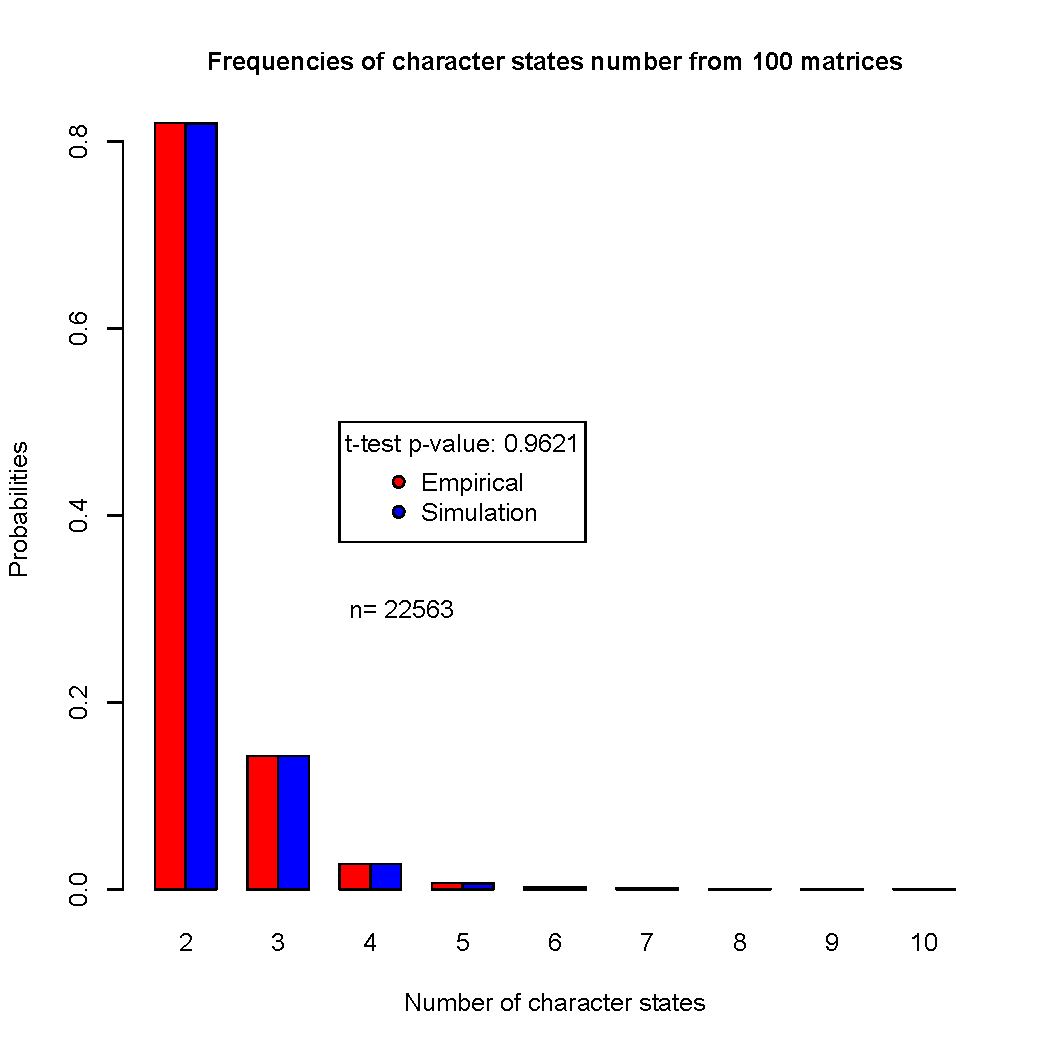
\includegraphics[keepaspectratio=true]{Figures/TEM_Fig-AppendixCharacters.pdf}
\caption{Character states distribution in empirical matrices. %Title?
Characters states number distribution extracted from 100 random morphological matrices downloaded from RreeBase.}
\label{Fig_AppendixCharacters}
\end{figure}

\subsection{Tree Building Software settings}

\subsubsection{Maximum Likelihood - RAxML v8.0.20 \citep{Stamatakis21012014}} \\
Model: \\
Molecular data: \\
GTR + $\Gamma_4$ (-m GTRGAMMA) \\
Morphological data: \\
Mk + $\Gamma_4$ (-K MK) \\
Support: \\
Rapid Boostrap algorithm (LSR), 1000 replicates \\

\subsubsection{Bayesian - MrBayes v3.0.2 \citep{Ronquist2012mrbayes}} \\
Priors: \\
Molecular data: \\
rates distribution shape ($\alpha$) = 0.5 \\
Transition/Transversion ratio = 2 ($\beta$(80,40)) \\
Starting tree: "True" tree topology with each branch length = 1 \\
Morphological data: \\
rates distribution shape ($\alpha$) = 0.5 \\
Models: \\
Molecular data: HKY + $\Gamma_4$ \\
Morphological data: Mk + $\Gamma_4$ \\
MCMC: \\
2 runs \\
4 chains per run \\
generations < 50$\times$$1^6$ \\
sample frequency = 1050$\times$$1^3$ \\
ASDS diagnosis frequency = 50$\times$$1^3$ \\
ASDS $<$ 0.01 \\
ESS $>>$ 200 \\
Burnin = 25\%

\subsection{Triplets metric details ($T_{x,y}$)}
Each triplet can be written as $I_{ijk}$=(\textit{ijk})). Where $I_{ijk}$ is equal to 0 if the the two triplets (\textit{ijk}) are the same in the two trees otherwise $I_{ijk}$ is equal to 1.
For any rooted tree there are only four possible combinations per triplets: ((\textit{j},\textit{k}),\textit{i});, ((\textit{i},\textit{k}),\textit{j}); and ((\textit{i},\textit{j}),\textit{k}); and (\textit{i},\textit{j},\textit{k}); \citep{johnson1998}.
One can calculate $S_n$, the triplet distance between two trees as:
\begin{equation}
S_n = \sum_{ijk} I_{ijk}
\end{equation}
Where:
\begin{equation}
\sum_{ijk} = \binom{n}{4} = \frac{n!}{4!(n-4)!}
\end{equation}
And where n is the number of taxa in both trees (modified from \citet{critchlowthe1996}).
When all triplets across the two trees are the same, $S_n$ is equal to 0 and when all the triplets are different $S_n$ is equal to $\binom{n}{4}$.
Because the possible number of triplets per clade is a finite number, the probability of two random trees with the same n taxa to have the same triplet is:
\begin{equation}
P({I_{ijk}}=0) = \frac{1}{4}
\end{equation}
Therefore one can calculate the probability of two random trees having the same triplets: 
\begin{equation}
P({S_{n}}=0) = \sum_{ijk} P_{I_{ijk}=0}
\end{equation}
\begin{equation}
P({S_{n}}=0) = \frac{n!}{4(3!(n-3)!}
\end{equation}
And in the same way:
\begin{equation}
P({S_{n}}=1) = \frac{3n!}{4(3!(n-3)!}
\end{equation}

\subsection{RF metric details}
The RF distance (or path difference) between two trees reflects the distance between the distributions of the tips among clades in the two trees \citep{RF1981} and can be expressed as following:
\begin{equation}
RF_{x,y} = N_{x} + N_{y} - 2C_{x,y}
\end{equation}
Where $C_{x,y}$ is the number of clades in common in the two trees. 
The minimal value of \textit{C} is equal to 1 if the two trees have the same n taxa;
the maximal value in \textit{C}=\textit{n}-2.
For a fully unresolved tree (star tree) \textit{N}=1 and for a fully resolved tree (binary tree) \textit{N}=\textit{n}-2.
The minimal and maximal topological distance for \textit{n} taxa is:
\begin{equation}
RF_{min} = 1 + 1 - 2C_{x,y}
\end{equation}
And:
\begin{equation}
RF_{max} = 2(n-2)-2
\end{equation}
One can then rescale \textit{RF.scaled} by using the maximal and minimal value for any \textit{n} taxa:
\begin{equation}
RF.scaled_{x,y} = \frac{RF_{x,y}-RF_{max}}{RF_{max}}
\end{equation}
This metric is more sensitive to taxa displacement than the Triplet distance \citep{critchlowthe1996,johnson1998,wiensmissing2003} and therefore a low value will show a good clade conservation between two trees and a high value will show a bad recovery of common clades.

\subsection{Tree comparisons}
\subsubsection{Random tree comparison scaling}
We used the comparison of 1000 random trees to obtain the mean comparison value $\bar{d}_{m,n}$\textit{(rand)} for the NTS metric.
We randomly generated two sets of 1000 trees of \textit{n} taxa using the rmtree function of ape package (v3.0-11 \citet{paradisape:2004}) that generates a given number of random Yule trees.
We calculated the $\bar{d}_{m,n}$\textit{(rand)} value using an approach similar to the RPCBTC (described below) by performing 1000 random pairwise comparisons using the TreeCmp java script \citep{Bogdanowicz2012}.

\subsubsection{Random Pairwise Bayesian Tree Comparison (RPBTC)}
We assessed the power of the Random Pairwise Bayesian Tree Comparison (RPBTC) method by comparing 1000 random trees from a posterior distribution trees set to another 1000 random trees from the same posterior distribution trees set.
We repeated this 100 times independently using the same posterior distribution trees set each time resulting in 100 replicates of the same posterior distribution trees set compared 1000 times.
We used an anova to test if there was no significant difference between the replicates so that the RBTC can be replicated.
We applied this protocol on a poorly resolved tree (Low Score), a resolved tree with low support value (Medium Score) and a resolved tree with high support values (High Score).
Results are available in table ~\ref{RPBTC_testing}. %link broken

\begin{table}[ht]
\caption{Group comparison results: difference between 100 replicates using the RPBTC method} %test with TreeCmp.anova
\centering
\begin{tabular}{rllrrrr}
  \hline
  Tree.Type & Used.metric & Replicates & Df & F.value & p.value \\ 
  \hline
  Low Score & RF & 100.00 & 99.00 & 0.74 & 0.98 \\ 
  Low Score & Tr & 100.00 & 99.00 & 0.97 & 0.58 \\ 
  Medium Score & RF & 100.00 & 99.00 & 0.64 & 1.00 \\ 
  Medium Score & Tr & 100.00 & 99.00 & 0.45 & 1.00 \\ 
  High Score & RF & 100.00 & 99.00 & 0.20 & 1.00 \\ 
  High Score & Tr & 100.00 & 99.00 & 0.37 & 1.00 \\ 
  \hline
\end{tabular}
\end{table}
\label{RPBTC_testing}

\subsection{Codes}
All codes are available at: $https://github.com/TGuillerme/Total\_Evidence\_Method-Missing\_data/tree/master/Functions$
The tree comparison results analysis can be repeated for more details at: $https://github.com/TGuillerme/Total\_Evidence\_Method-Missing\_data/tree/master/Analysis$ %fully running! Try it at home (5-10 minutes of data loading)!

\subsection{Full results}

\begin{table}
\caption{Tree similarity values per parameter in ML framework}
\centering
\begin{tabular}{rrlccccc}
    \hline
    Parameter & amount of    & metric & mode & 50\%CI &       & 95\%CI &       \\
              & missing data &        &      & lower  & upper & lower  & upper \\
    \hline
    $M_L$     & 0\%          & Robinson-Fould & 1 & NA  & NA & NA  & NA \\
              &              & Triples        & 1 & NA  & NA & NA  & NA \\
              & 10\%         & Robinson-Fould & 0.6714878 & 0.5692308  & 0.7894649 & 0.4689069  & 1.0361514 \\ %how many digits?
              &              & Triples        & 0.9424133 & 0.8683742  & 0.9998559 & 0.6121399  & 1.0635250 \\
              & 25\%         & Robinson-Fould & 0.5167595 & 0.4403147  & 0.6307692 & 0.2664429  & 0.8929104 \\
              &              & Triples        & 0.5599494 & 0.7084874  & 0.8105781 & 0.2912950  & 0.9990703 \\
              & 50\%         & Robinson-Fould & 0.4321852 & 0.3641026  & 0.5215627 & 0.2313246  & 0.6423846 \\
              &              & Triples        & 0.5143009 & 0.4197127  & 0.5991498 & 0.2991432  & 0.9104526 \\
              & 75\%         & Robinson-Fould & 0.3727090 & 0.3230769  & 0.4342249 & 0.2035474  & 0.5776286 \\
              &              & Triples        & 0.4449563 & 0.3385128  & 0.5329149 & 0.1929395  & 0.8551570 \\
    $M_L$     & 0\%          & Robinson-Fould & 1 & NA  & NA & NA  & NA \\
              &              & Triples        & 1 & NA  & NA & NA  & NA \\
              & 10\%         & Robinson-Fould & 0.9072419 & 0.7668415  & 1.0000000 & 0.4070844  & 1.0478010 \\
              &              & Triples        & 0.9763617 & 0.9448100  & 1.0039460 & 0.7158118  & 1.1043330 \\
              & 25\%         & Robinson-Fould & 0.5722382 & 0.4883560  & 0.6923077 & 0.3253239  & 0.9367467 \\
              &              & Triples        & 0.9370152 & 0.8207407  & 0.9938846 & 0.5394443  & 1.0868073 \\
              & 50\%         & Robinson-Fould & 0.4338159 & 0.3025641  & 0.4760777 & 0.1704016  & 0.6683220 \\
              &              & Triples        & 0.7327464 & 0.5947211  & 0.8739630 & 0.3418679  & 1.0251540 \\
              & 75\%         & Robinson-Fould & 0.1534487 & 0.1155128  & 0.2000000 & 0.0683485  & 0.3230769 \\
              &              & Triples        & 0.4588292 & 0.3905631  & 0.6111484 & 0.2903676  & 0.8568274 \\   
    $M_L$     & 0\%          & Robinson-Fould & 1 & NA  & NA & NA  & NA \\
              &              & Triples        & 1 & NA  & NA & NA  & NA \\
              & 10\%         & Robinson-Fould & 0.473285 & 0.3842965  & 0.8358974 & 0.3564753  & 0.9589744 \\
              &              & Triples        & 0.9592557 & 0.8691580  & 1.026095 & 0.5720847  & 1.067524 \\
              & 25\%         & Robinson-Fould & 0.4548038 & 0.3572132  & 0.6307692 & 0.2425339  & 0.9161212 \\
              &              & Triples        & 0.9071925 & 0.7516934  & 0.9976224 & 0.4462168  & 1.0705291 \\
              & 50\%         & Robinson-Fould & 0.4244263 & 0.3755493  & 0.4666667 & 0.2494927  & 0.8287312 \\
              &              & Triples        & 0.6834366 & 0.5713927  & 0.8226139 & 0.2776690  & 1.0085944 \\
              & 75\%         & Robinson-Fould & 0.2306888 & 0.1774508  & 0.3025641 & 0.1087764  & 0.5673541 \\
              &              & Triples        & 0.4513642 & 0.3737397  & 0.5723858 & 0.2245224  & 0.7917946 \\
    \hline
\label{NTSML_full}
\end{tabular}
\end{table}

\begin{table}
\caption{Tree similarity values per parameter in Bayesian framework}
\centering
\begin{tabular}{rrlccccc}
    \hline
    Parameter & amount of    & mode & 50\%CI &       & 95\%CI & \\
              & missing data &      & lower  & upper & lower  & upper \\
    \hline
    $M_L$     & 0\%          & Robinson-Fould & 0.05641026 & 0.03589744  & 0.06337695 & 0.03139209  & 0.07692308 \\ %how many digits?
              &              & Triples        & 0.04104231 & 0.00830962  & 0.05441173 & -0.03933377  & 0.10690054 \\
              & 10\%         & Robinson-Fould & 0.03584309 & 03584196  & 03589744 & 02825643  & 0.06175676 \\
              &              & Triples        & 0.03399849 & 0.003196469  & 0.04981018 & -0.049913382  & 0.11784366 \\
              & 25\%         & Robinson-Fould & 0.03589744 & 0.03589744  & 0.03589744 & 0.01536739  & 0.06123106 \\
              &              & Triples        & 0.03510953 & 0.002113358  & 0.04939228 & -0.041202264  & 0.09699332 \\
              & 50\%         & Robinson-Fould & 0.03589744 & 0.03589744  & 0.03589744 & 0.01538462  & 0.05641026 \\
              &              & Triples        & 0.02849433 & 0.003263098  & 0.05298036 & -0.038344731  & 0.09250063 \\
              & 75\%         & Robinson-Fould & 0.03589744 & 0.03589744  & 0.03589744 & 0.01069992  & 0.04338811 \\
              &              & Triples        & -0.0001940566 & -0.01801301  & 0.04058783 & -0.06030922  & 0.10665934 \\
    $M_L$     & 0\%          & Robinson-Fould & 0.05641026 & 0.03589744  & 0.06337695 & 0.03139209  & 0.07692308 \\
              &              & Triples        & 0.04104231 & 0.008309622  & 0.05441173 & -0.039333778  & 0.10690054 \\
              & 10\%         & Robinson-Fould & 0.03593712 & 0.03198256  & 0.05641026 & 0.02798864  & 0.07692308 \\
              &              & Triples        & 0.02639309 & 0.002185408  & 0.05061314 & -0.046563042  & 0.10547052 \\
              & 25\%         & Robinson-Fould & 0.03588134 & 0.03587629  & 0.03589744 & 0.01538462  & 0.0680884 \\
              &              & Triples        & 0.03856296 & 0.002185408  & 0.05061314 & -0.046563042  & 0.10547052 \\
              & 50\%         & Robinson-Fould & 0.03589744 & 0.03589744  & 0.03589744 & 0.01536289  & 0.05879269 \\
              &              & Triples        & 0.01403716 & -0.01100608  & 0.03972324 & -0.03800324  & 0.12405207 \\
              & 75\%         & Robinson-Fould & 0.03589206 & 0.03588825  & 0.03589744 & 0.01538462  & 0.0411843 \\
              &              & Triples        & 0.02939363 & 0.01902351  & 0.04238907 & -0.03087905  & 0.08946917 \\   
    $M_L$     & 0\%          & Robinson-Fould & 0.05641026 & 0.03589744  & 0.06337695 & 0.03139209  & 0.07692308 \\
              &              & Triples        & 0.04104231 & 0.008309622  & 0.05441173 & -0.039333778  & 0.10690054 \\
              & 10\%         & Robinson-Fould & 0.05637057 & 0.03589744  & 0.05927956 & 0.02813296  & 0.07692308 \\
              &              & Triples        & 0.03008132 & 0.01176800  & 0.04847400 & -0.02451461  & 0.09453754 \\
              & 25\%         & Robinson-Fould & 0.03593743 & 0.03589744  & 0.03596018 & 0.02330790  & 0.07692308 \\
              &              & Triples        & 0.02010221 & -0.001145118  & 0.0377779 & -0.060183332  & 0.1098632 \\
              & 50\%         & Robinson-Fould & 0.03589744 & 0.03589744  & 0.03589744 & 0.03050289  & 0.05950426 \\
              &              & Triples        & 0.01053959 & -0.005595947  & 0.04510444 & -0.036278820  & 0.10478805 \\
              & 75\%         & Robinson-Fould & 0.03589744 & 0.03589744  & 0.03589744 & 0.01115983  & 0.04362927 \\
              &              & Triples        & 0.02427778 & 0.0007405737  & 0.04260522 & -0.0373004106  & 0.1048756 \\
\label{NTSBA_full}
\end{tabular}
\end{table}

\subsection{Bootstraps distribution}

\begin{figure}
\centering
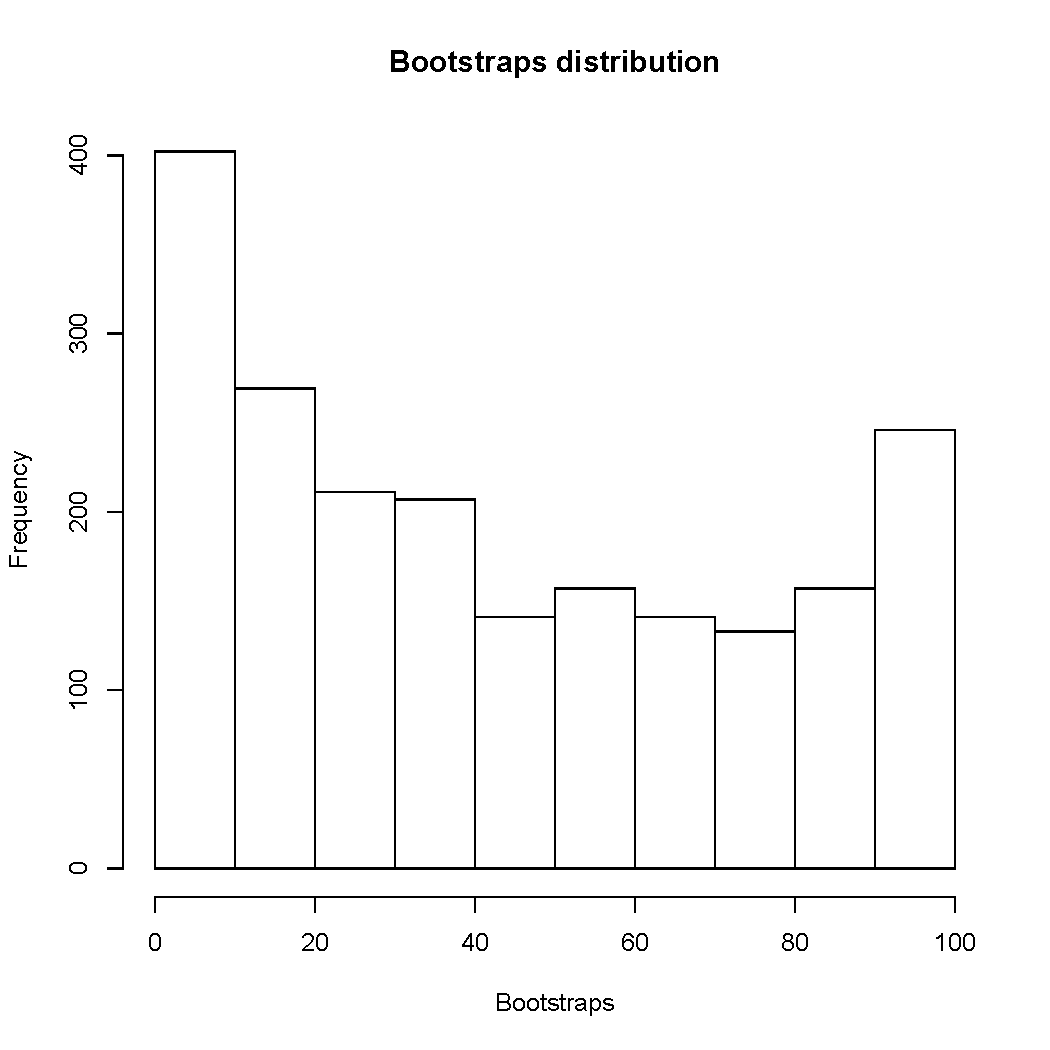
\includegraphics[keepaspectratio=true]{Figures/TEM_Fig-AppendixBootstraps.pdf}
\caption{Bootstraps distribution across the "best" trees.}                     % MISSING 8 CHAINS
\label{Fig_AppendixBoostraps}
\end{figure}


%END
\end{document}